\section{实验结果}
\subsection{对于高斯过程训练以及预测的效率方面的讨论}

\subsubsection{高斯过程与稀疏高斯过程在长期预测方面的对比}

\begin{figure}[!htbp]
    \centering
    \includegraphics[width=\textwidth]{images/lab1/HPQ_trend.png}
    \caption{HPQ长期趋势}\label{1lab1HPQtrend}
\end{figure}

如图\ref{1lab1HPQtrend}所示,采用与原始数据集样本数量相同的伪数据的$sgp\_100$模型在整体上最贴合实际走势。
而高斯回归模型$gp$和其余使用较少伪数据的$sgp\_10$都呈现朝均值衰减的趋势。


\begin{figure}[!htbp]
    \centering
    \begin{minipage}[t]{0.49\textwidth}
    \centering
    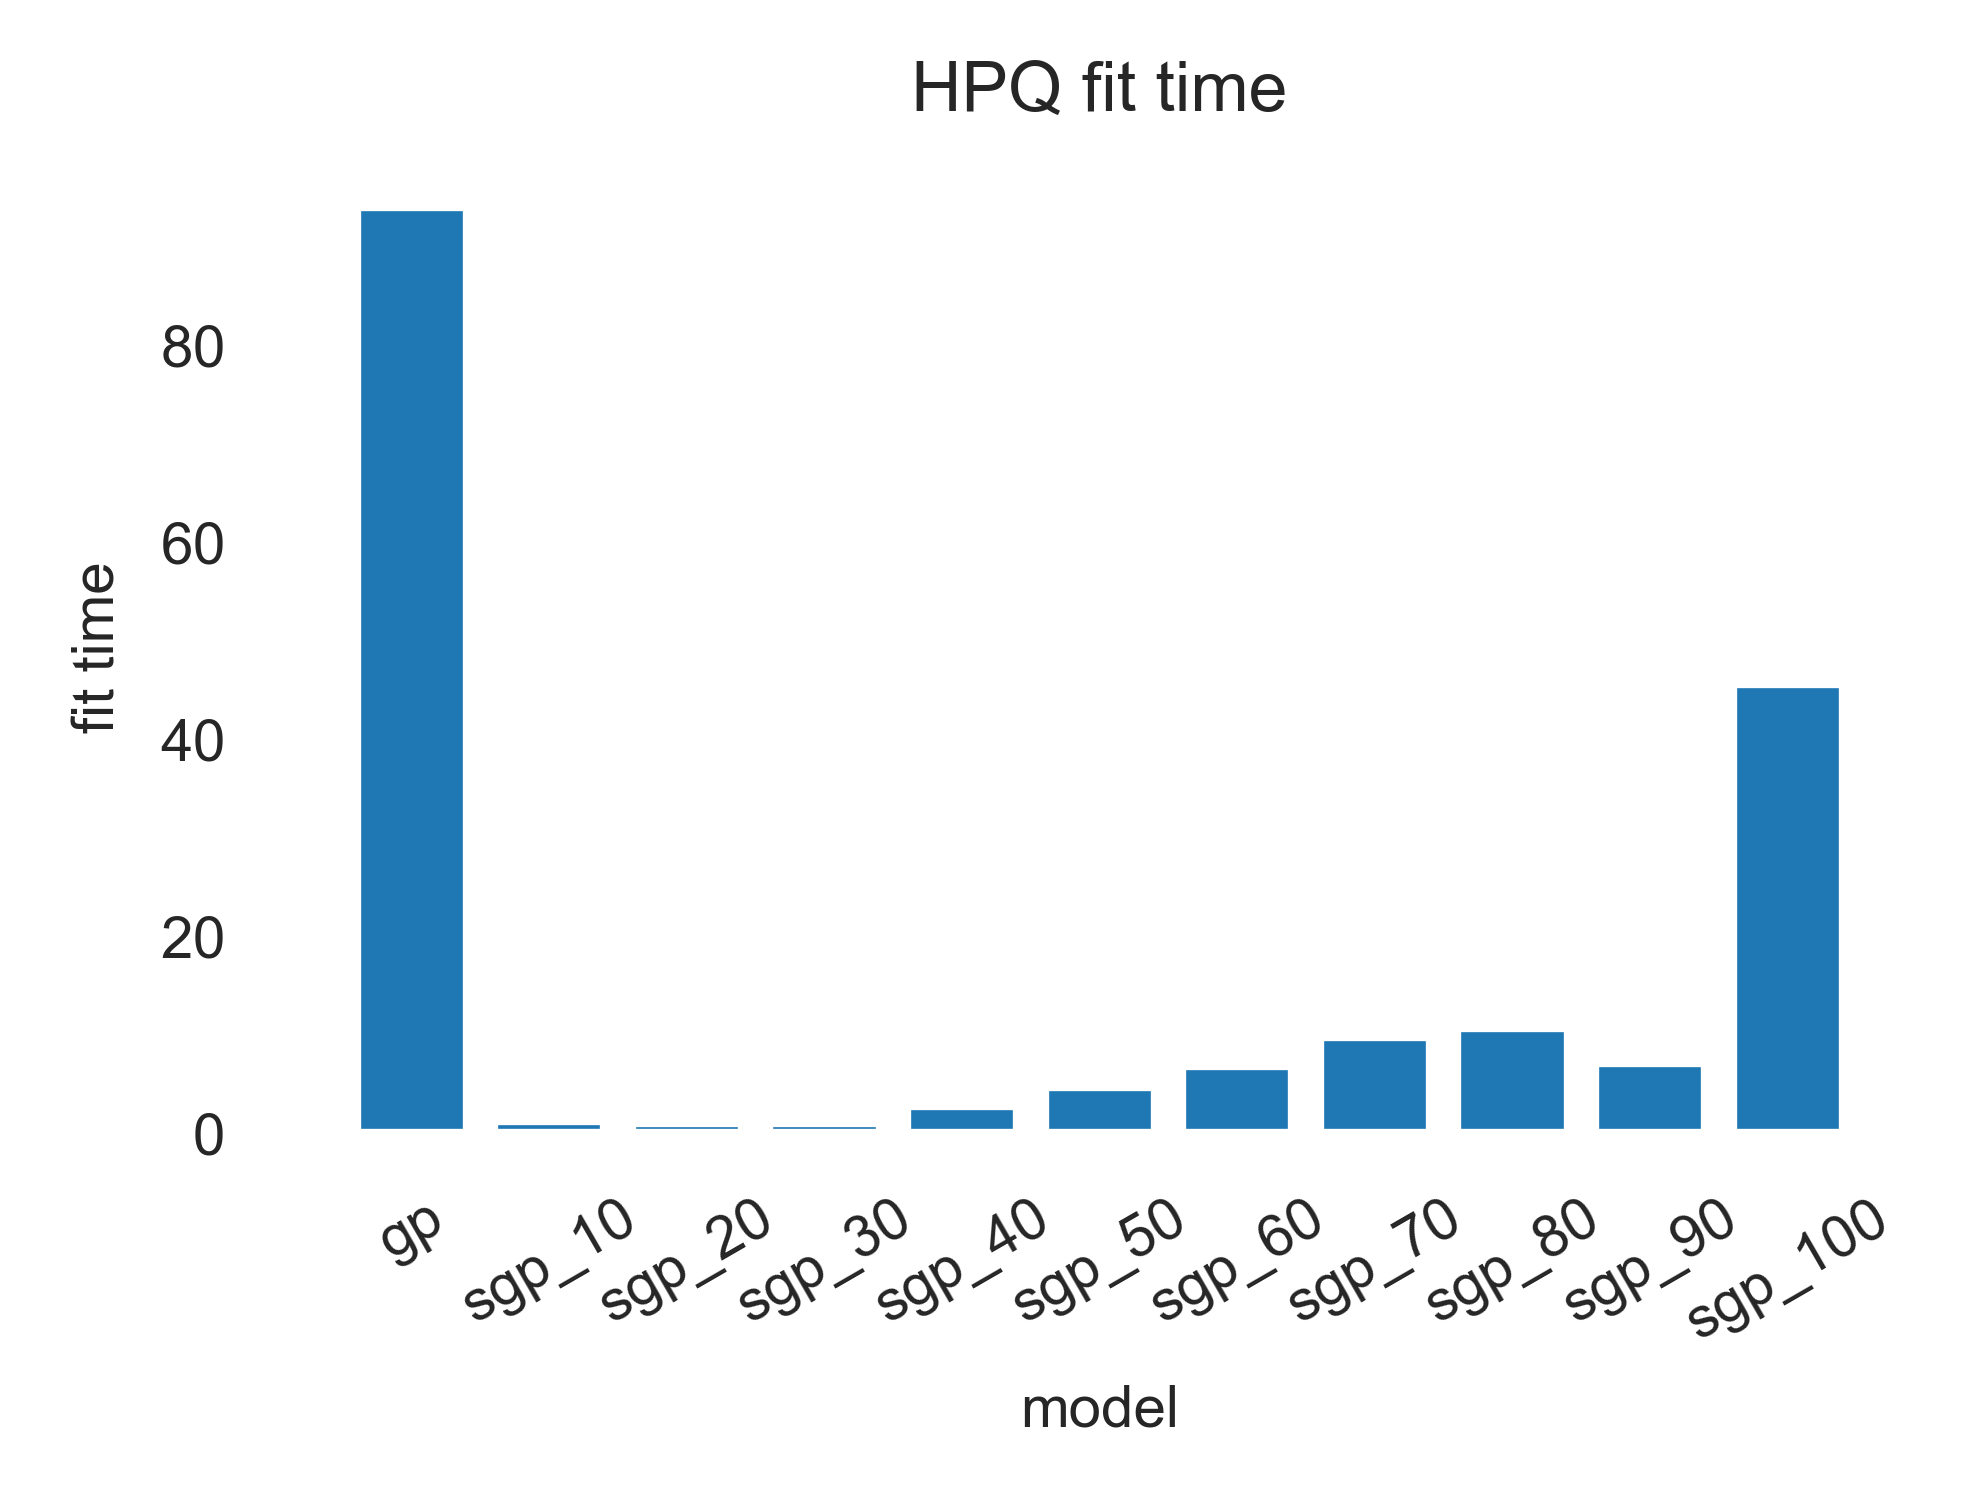
\includegraphics[width=\textwidth]{images/lab1/HPQ_fit_time.png}
    \caption{模型长期预测HPQ时的训练时间}\label{1HPQfittime}
    \end{minipage}
    \begin{minipage}[t]{0.49\textwidth}
    \centering
    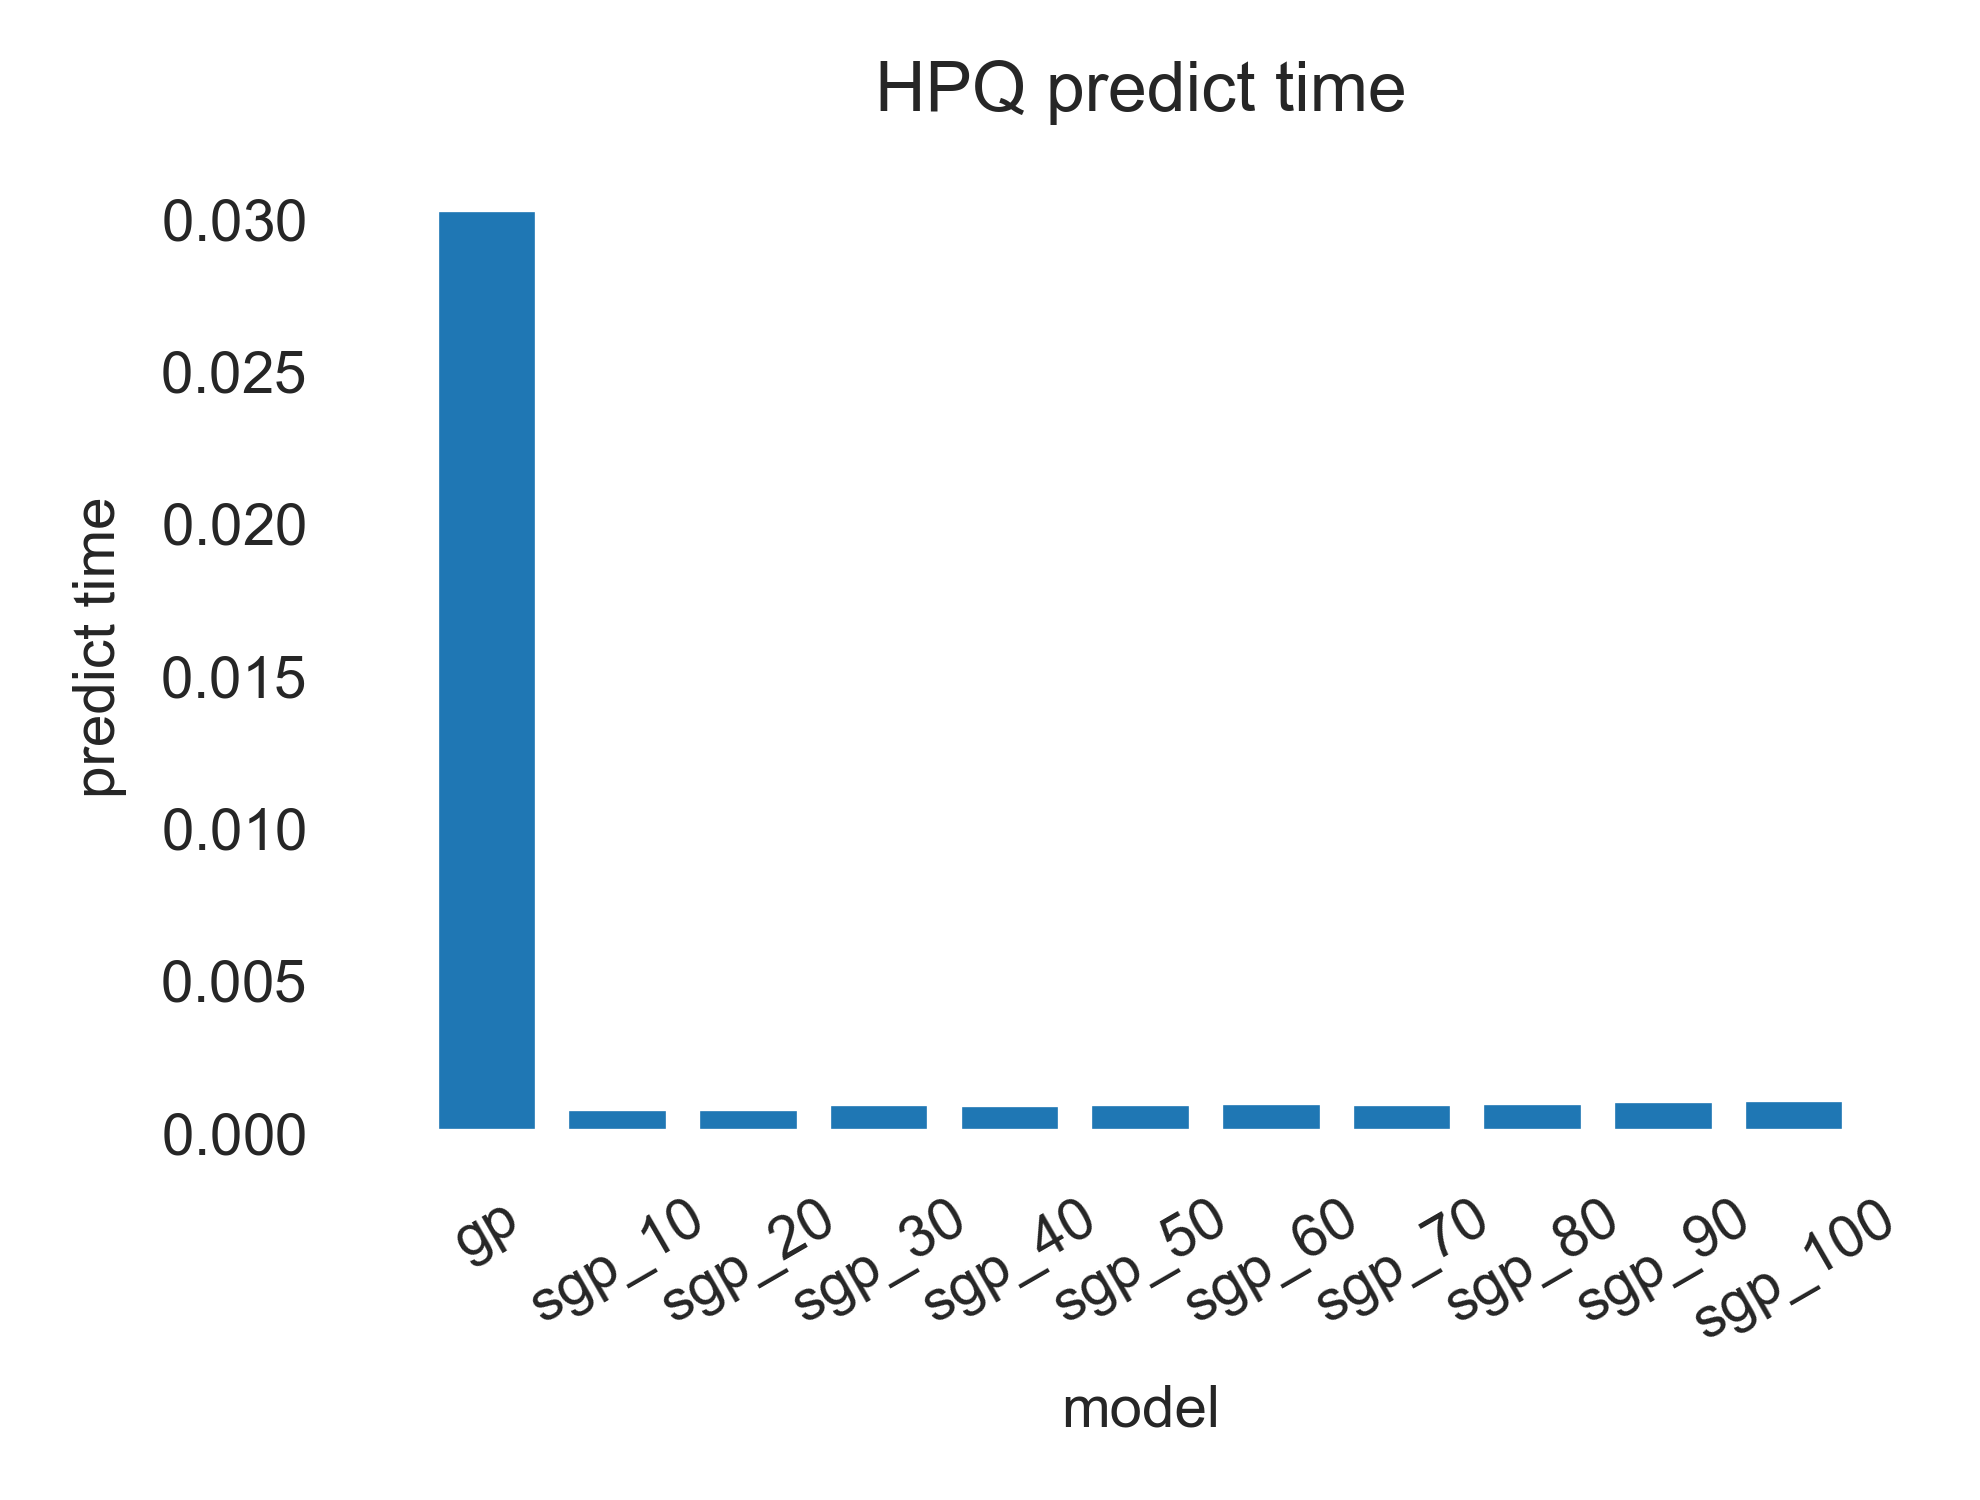
\includegraphics[width=\textwidth]{images/lab1/HPQ_predict_time.png}
    \caption{模型长期预测HPQ时的推理时间}\label{1HPQpredicttime}
    \end{minipage}
\end{figure}

从\ref{1HPQpredicttime},\ref{1HPQfittime}可以看出,稀疏高斯过程无论是在训练时间还是在预测时间上,都体现出强大的优势。
即使采用的伪数据的数量为原始数据集的数据数量,所需要时间也远小于原始的高斯过程。


\begin{figure}[!htbp]
    \centering
    \includegraphics[width=\textwidth]{images/lab1/VZ_trend.png}
    \caption{VZ长期趋势}\label{1lab1VZtrend}
\end{figure}

从图\ref{1lab1VZtrend}可以看出,采用与原始数据集样本数量相同的伪数据的$sgp\_100$模型在整体上最贴合实际走势。
其余使用较多伪数据的稀疏高斯模型也和$sgp\_100$呈现出先上升再下降的趋势;而$gp$和使用较少伪数据的稀疏高斯模型则呈现出
朝均值递减的趋势。

\begin{figure}[!htbp]
    \centering
    \begin{minipage}[t]{0.49\textwidth}
    \centering
    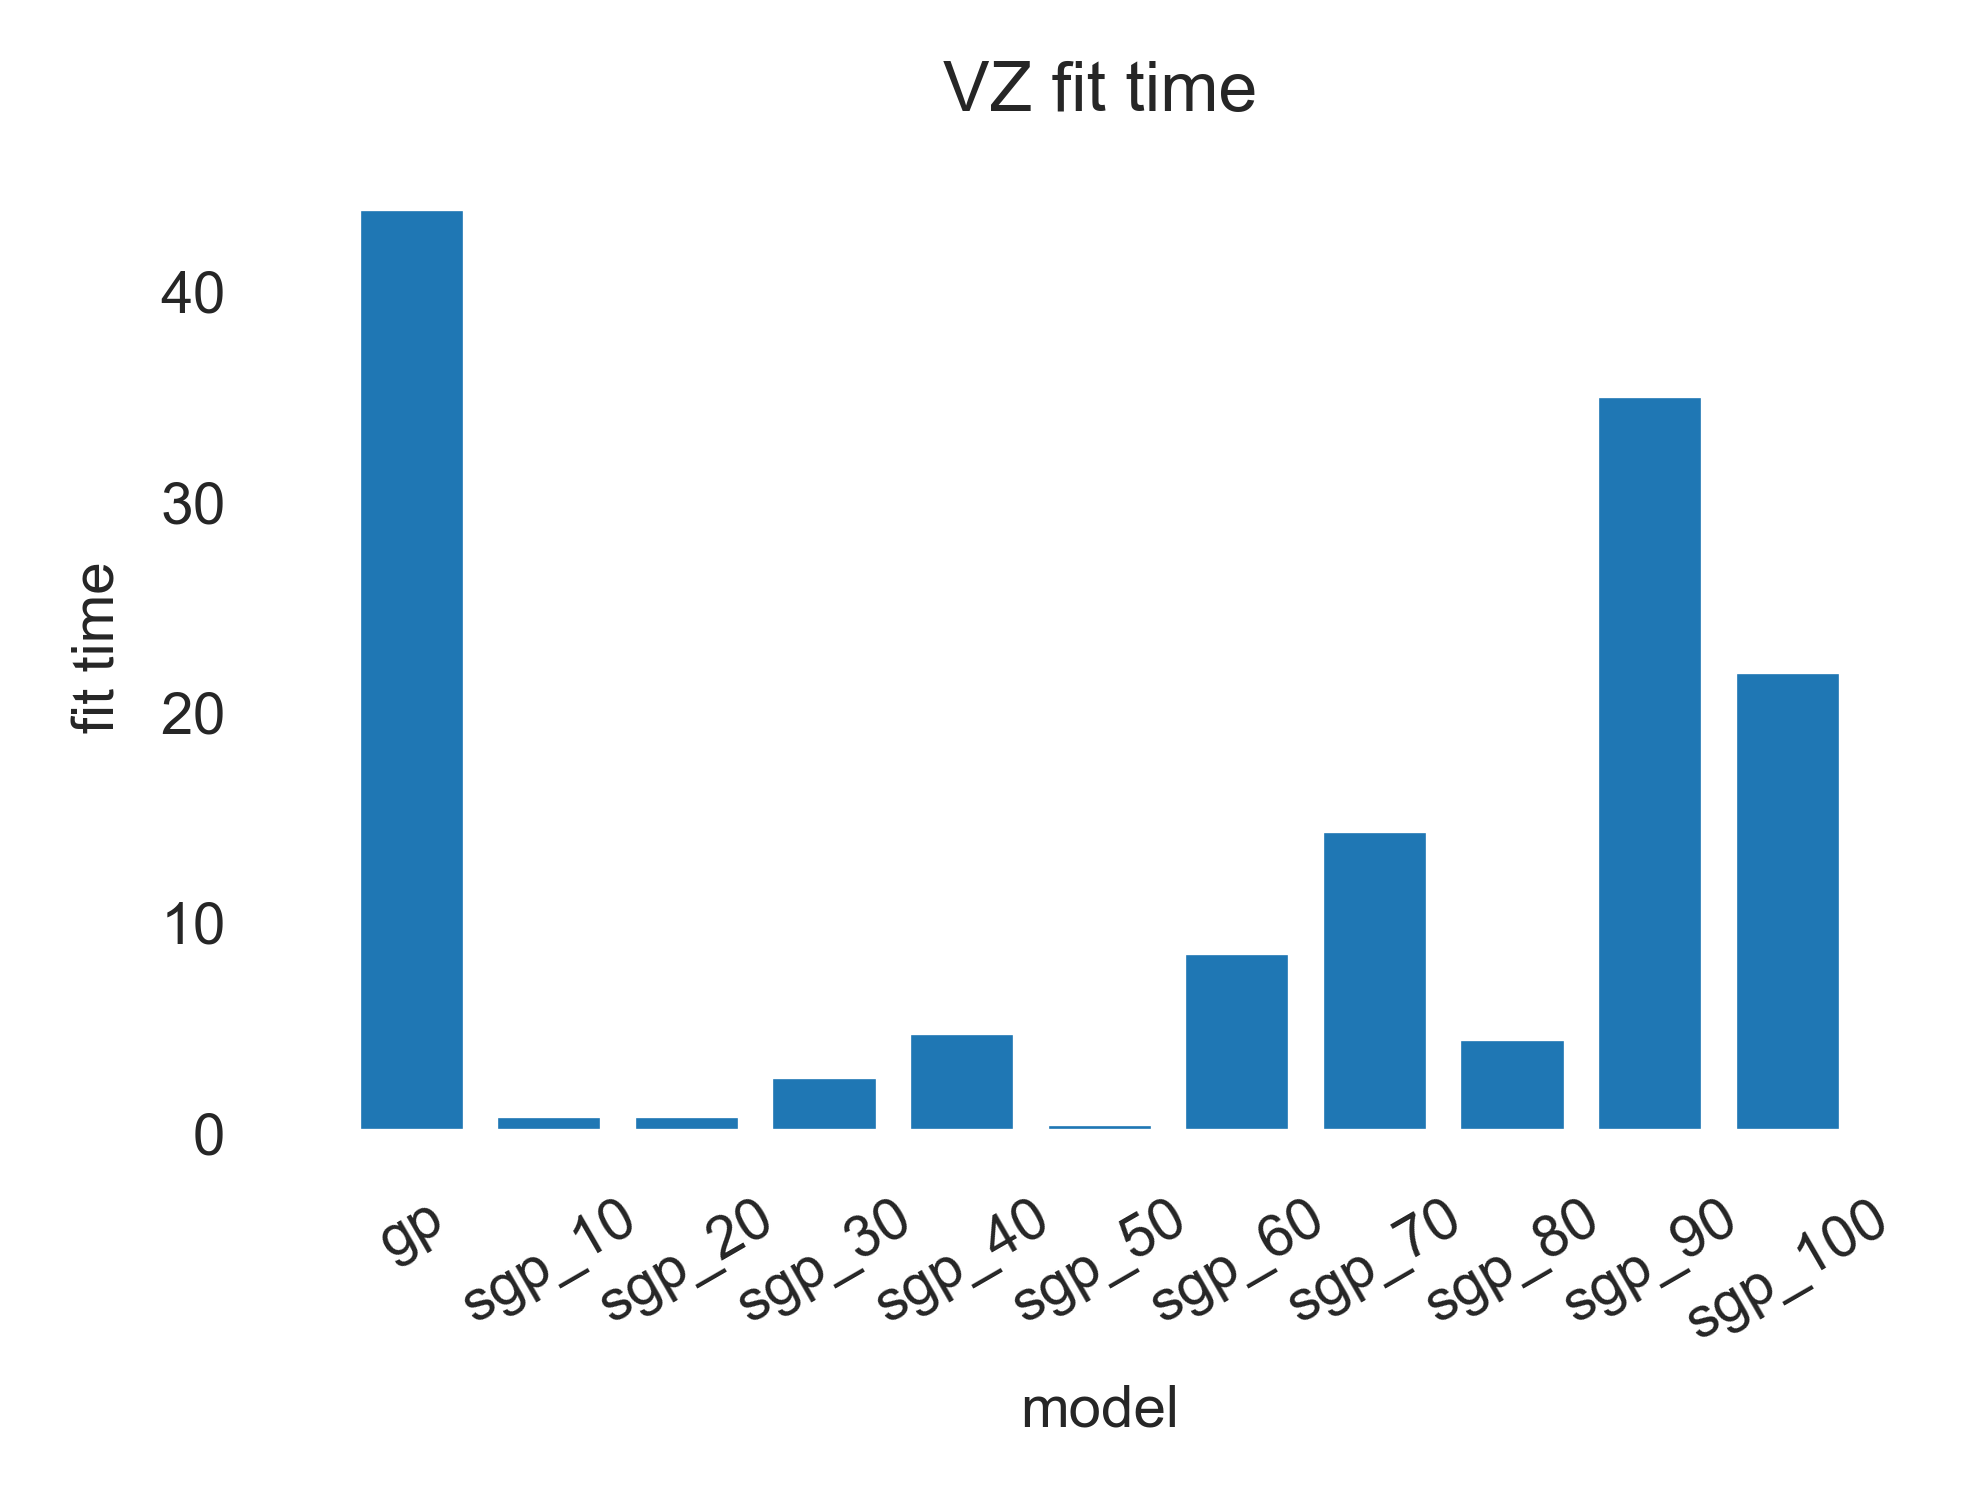
\includegraphics[width=\textwidth]{images/lab1/VZ_fit_time.png}
    \caption{模型长期预测VZ时的训练时间}\label{1VZfittime}
    \end{minipage}
    \begin{minipage}[t]{0.49\textwidth}
    \centering
    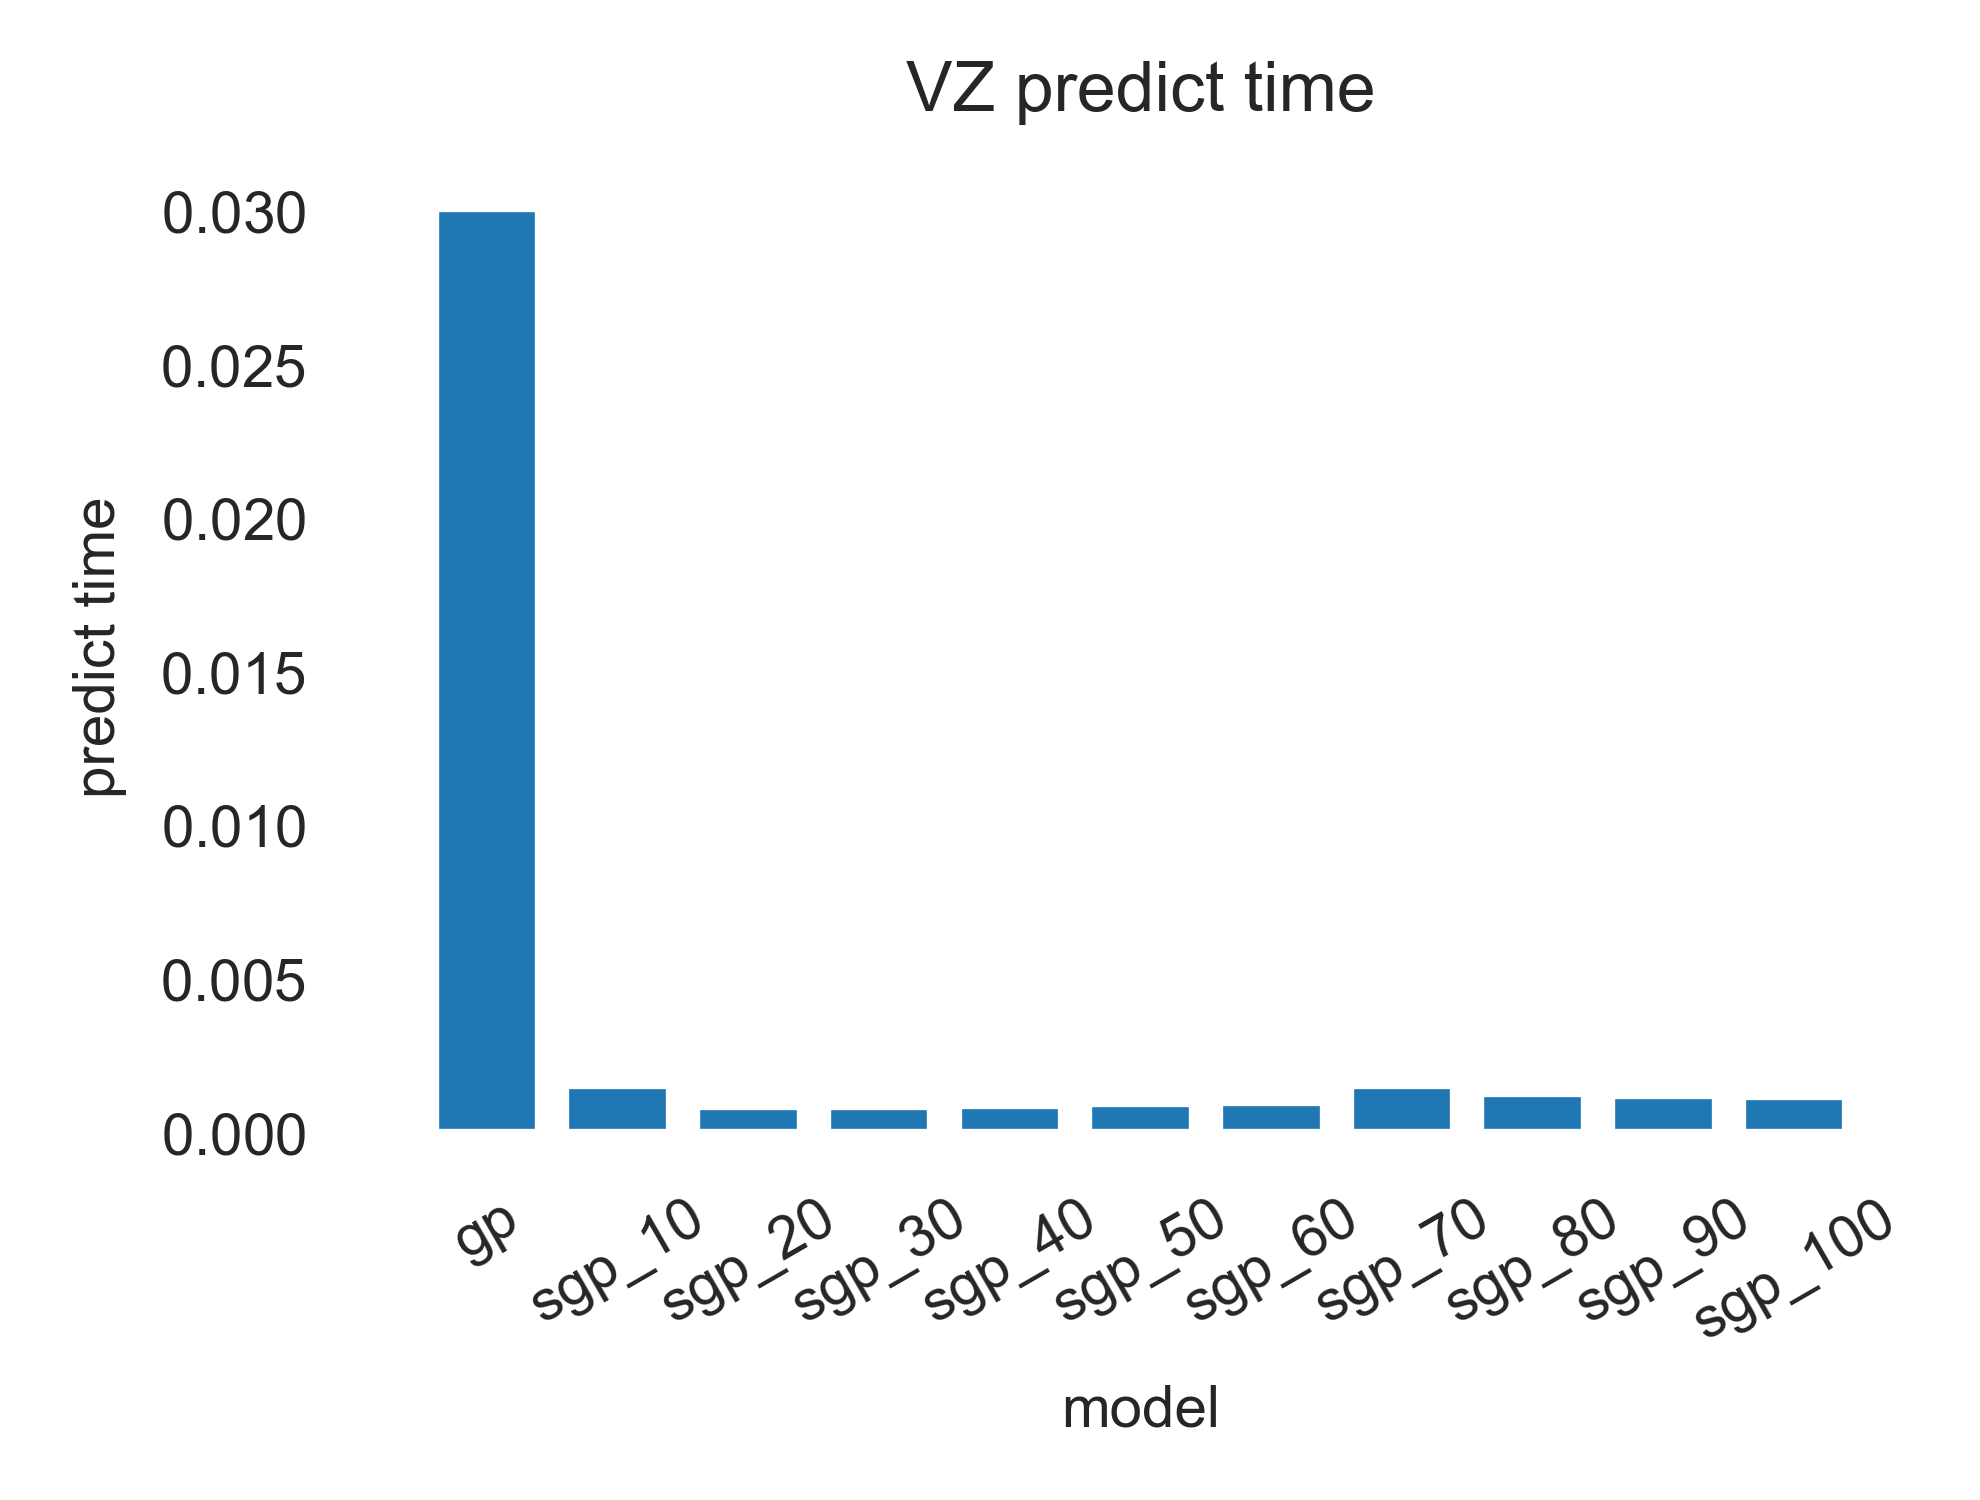
\includegraphics[width=\textwidth]{images/lab1/VZ_predict_time.png}
    \caption{模型长期预测VZ时的推理时间}\label{1VZpredicttime}
    \end{minipage}
\end{figure}



从图\ref{1VZfittime},\ref{1VZpredicttime}可以看出,稀疏高斯过程训练以及预测所需的时间并不是严格和所用伪数据的大小成正比的,
其原因可能在于稀疏高斯过程可能会额外对伪数据的分布进行优化,而这一部分所需的时间不严格和所用伪数据的大小成正比。


\begin{figure}[!htbp]
    \centering
    \includegraphics[width=\textwidth]{images/lab1/SBUX_trend.png}
    \caption{SBUX长期趋势}\label{1lab1SBUXtrend}
\end{figure}

从图\ref{1lab1SBUXtrend}中可以看出,大部分模型所给出来的预测偏差幅度大,其中包括高斯过程模型$gp$。
而采用较多伪数据的稀疏高斯过程$sgp\_100$和$sgp\_90$则在前期对于趋势刻画的比较好。

\begin{figure}[!htbp]
    \centering
    \begin{minipage}[t]{0.49\textwidth}
    \centering
    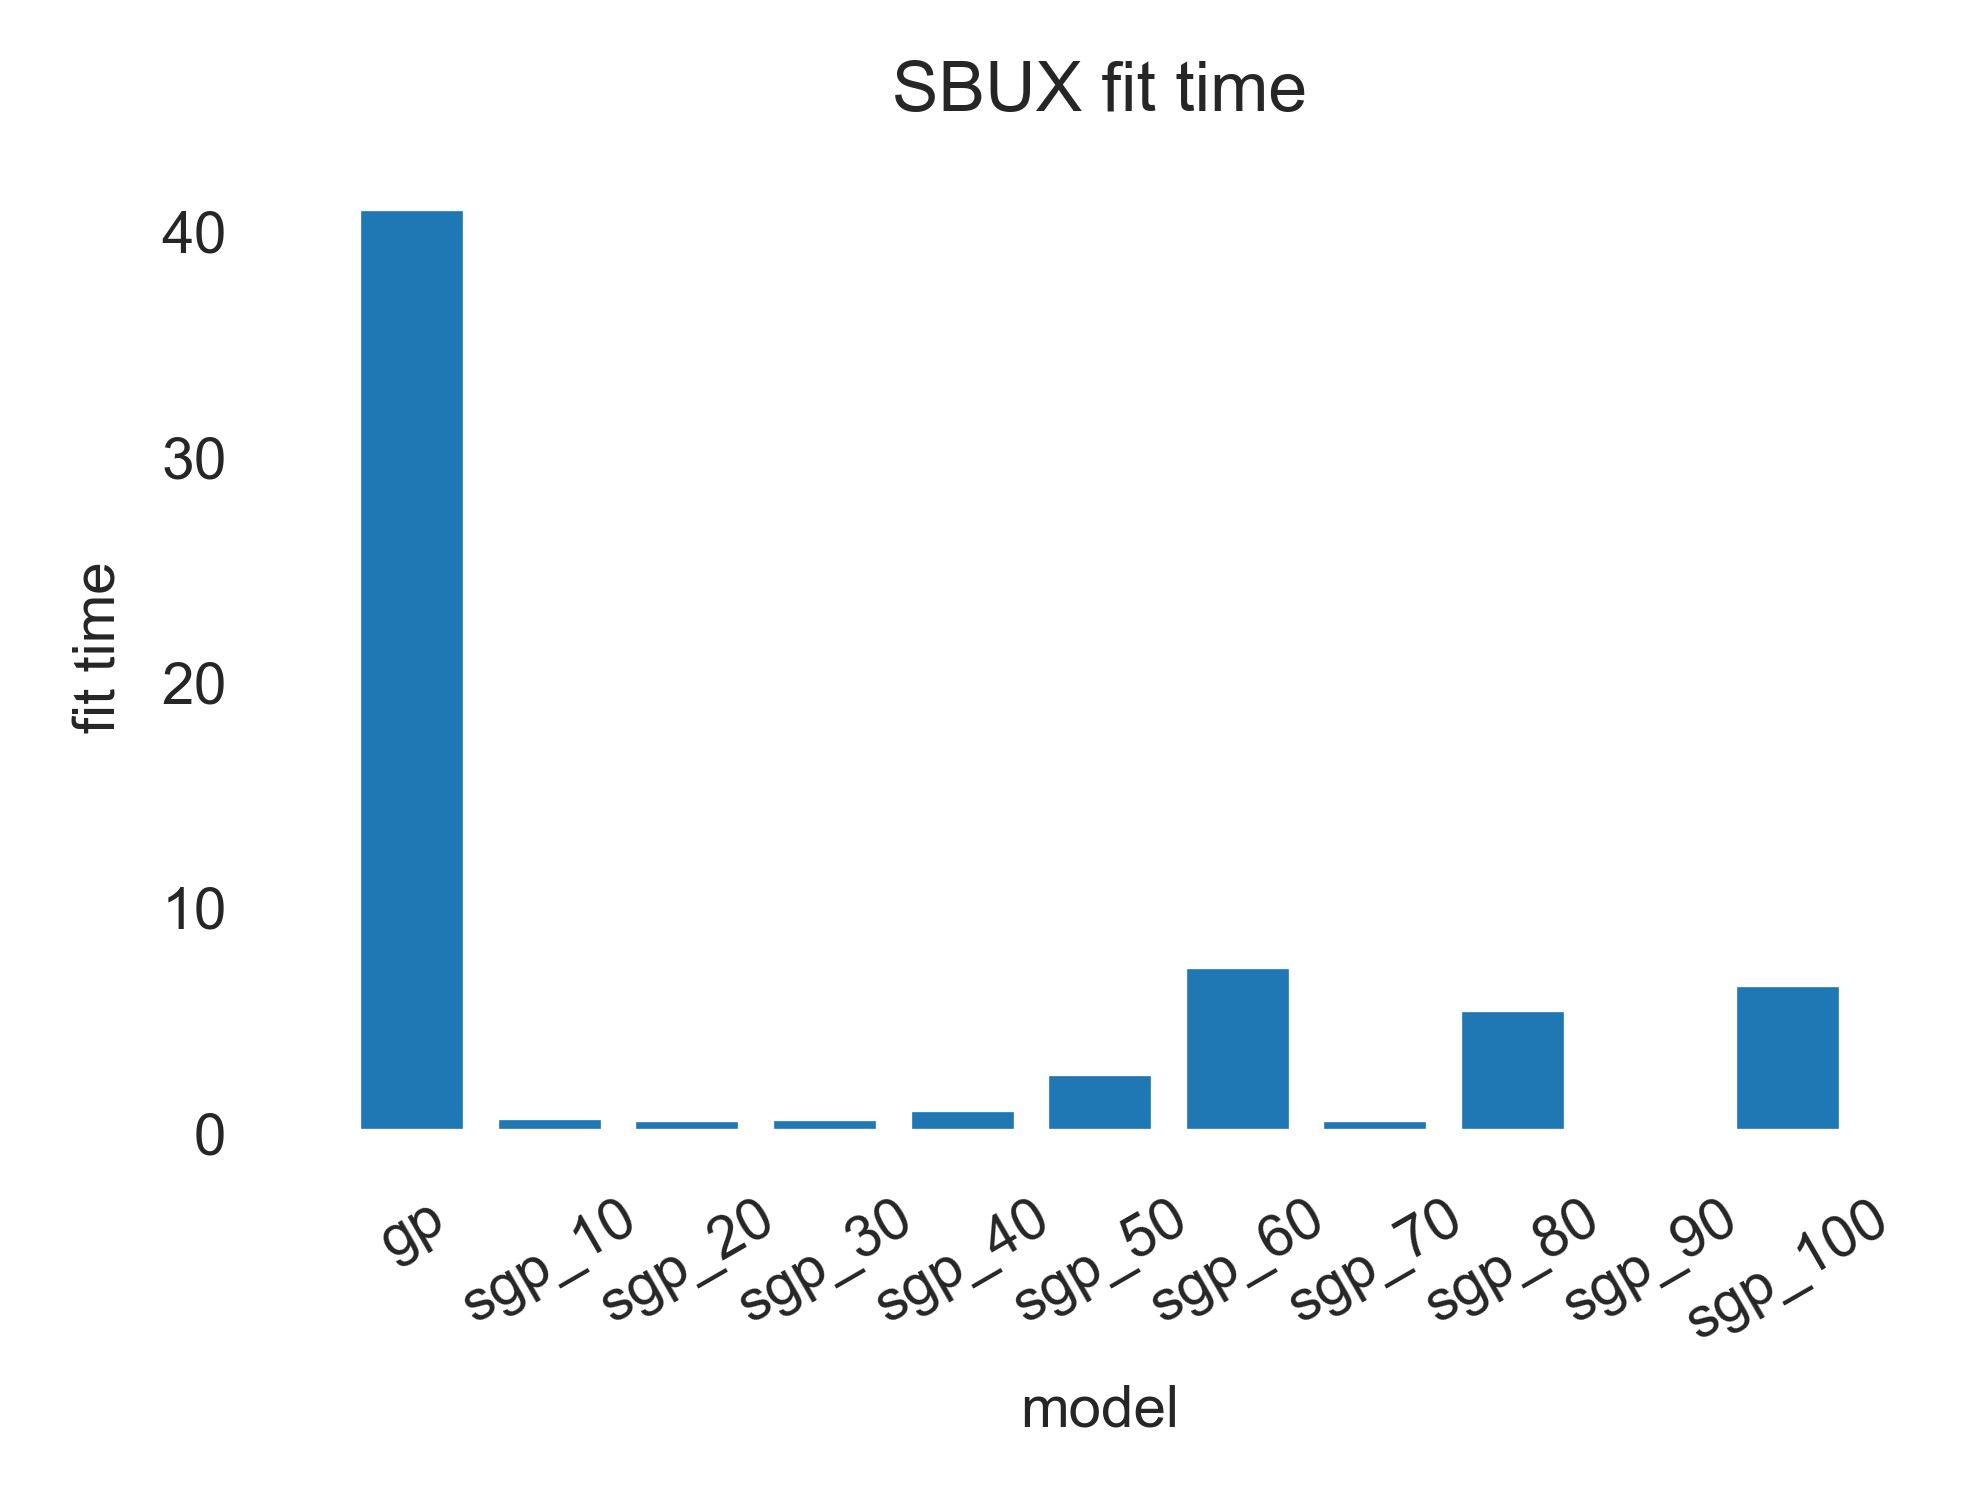
\includegraphics[width=\textwidth]{images/lab1/SBUX_fit_time.png}
    \caption{模型长期预测SBUX时的训练时间}\label{1SBUXfittime}
    \end{minipage}
    \begin{minipage}[t]{0.49\textwidth}
    \centering
    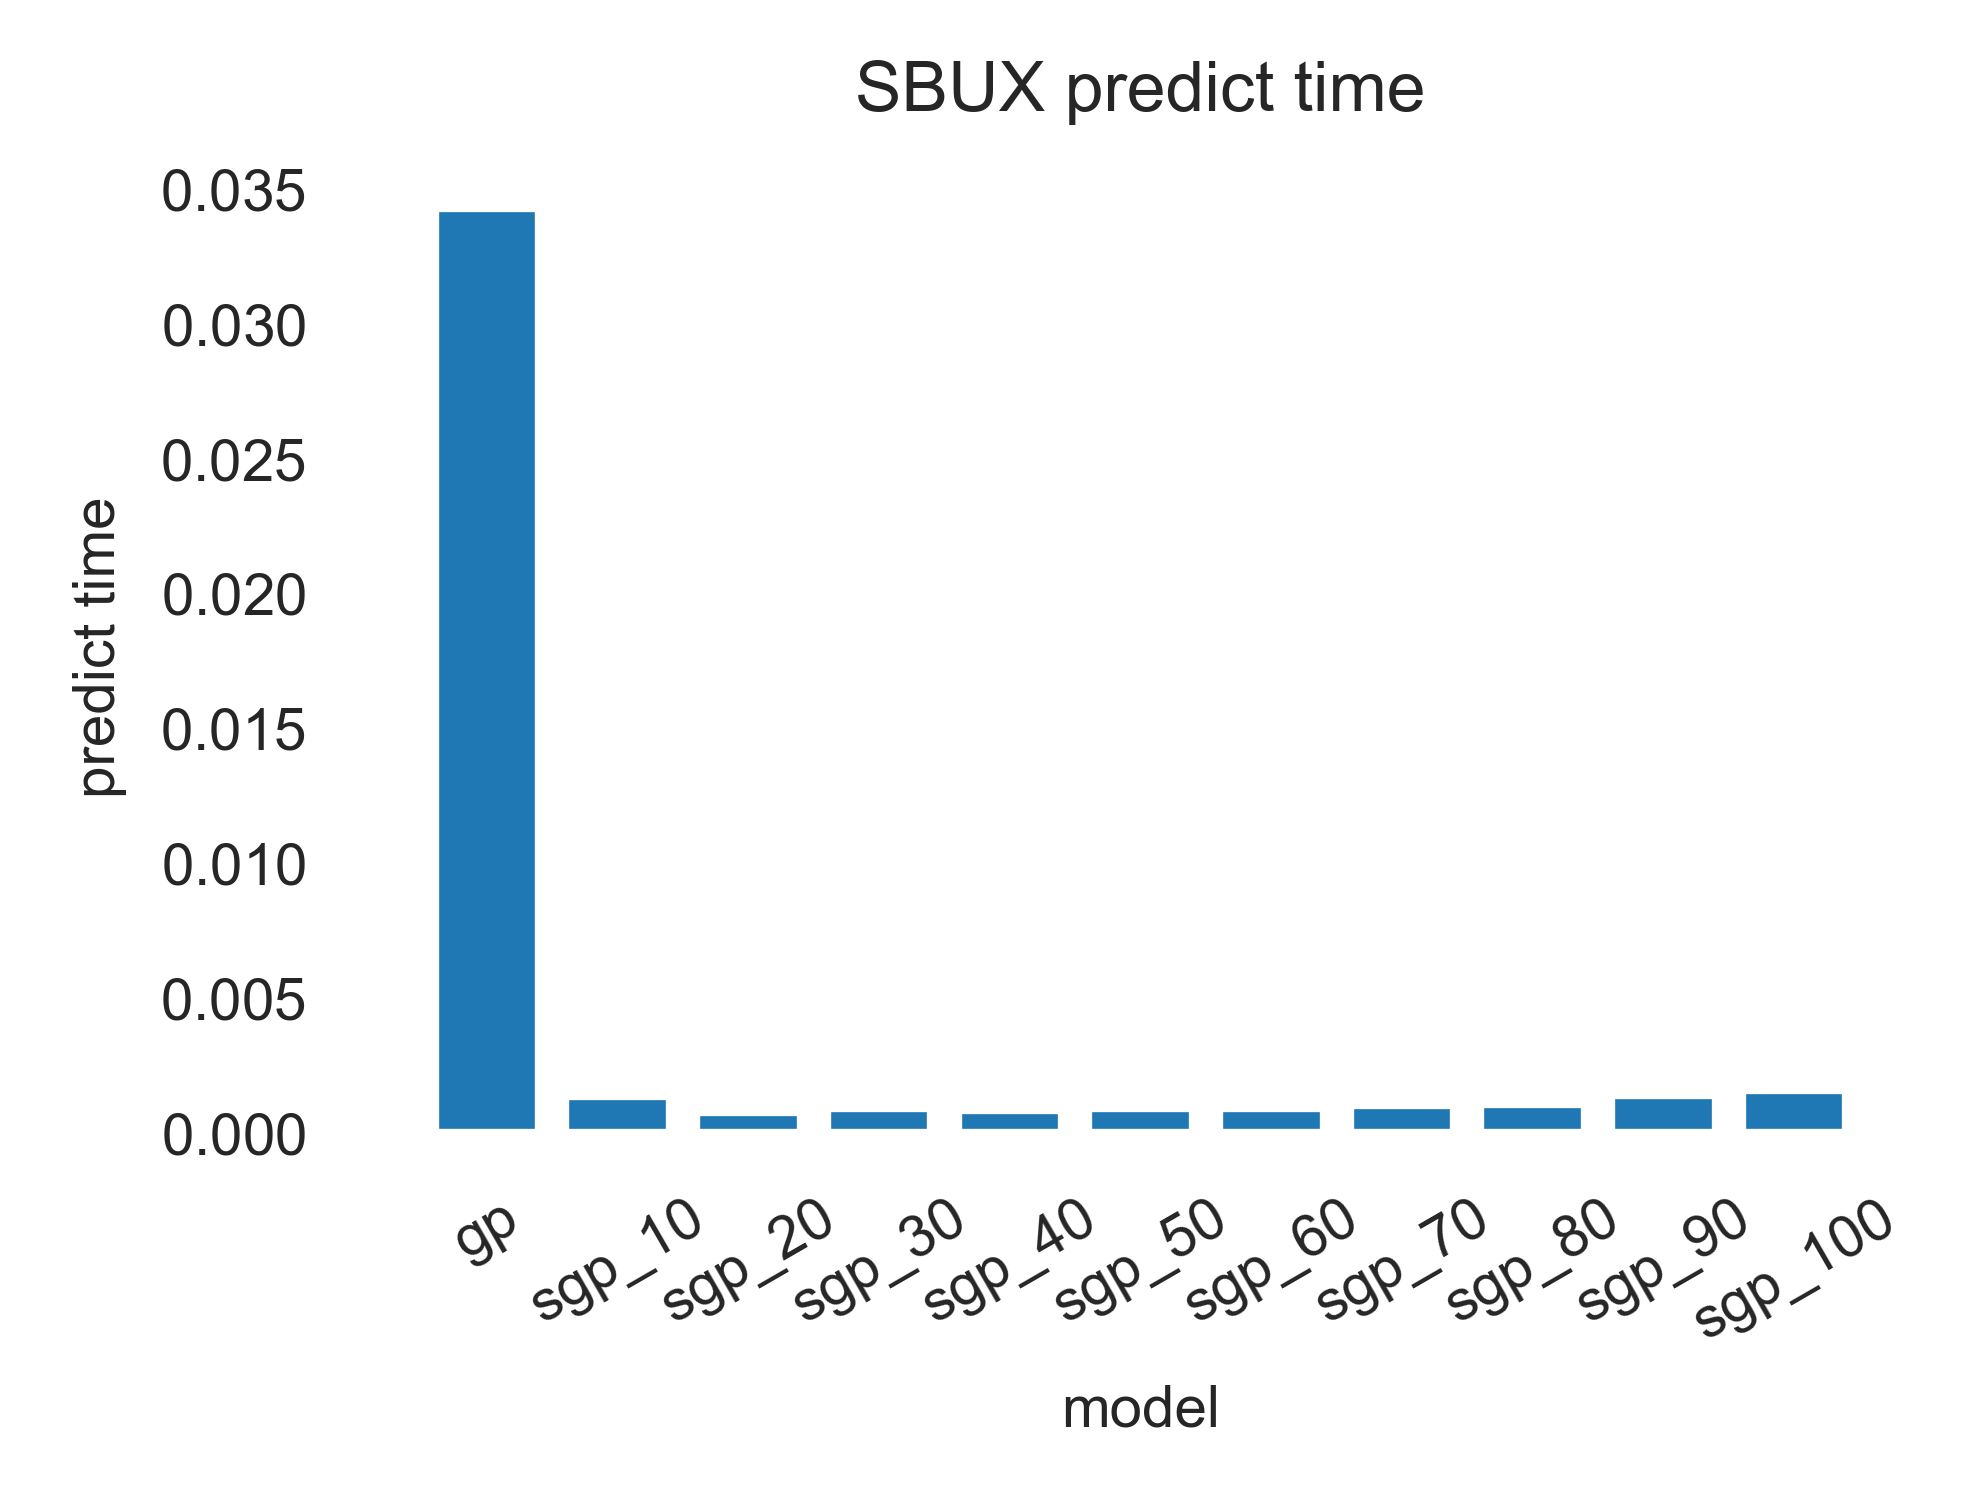
\includegraphics[width=\textwidth]{images/lab1/SBUX_predict_time.png}
    \caption{模型长期预测SBUX时的推理时间}\label{1SBUXpredicttime}
    \end{minipage}
\end{figure}

\subsubsection{训练集大小对于高斯过程长期预测能力的影响}

从图\ref{2lab2HPQtrend}中可以看出,除了只使用$10\%$的训练集得到的高斯过程模型$gp\_10$外,其余的高斯过程模型所给出的长期预测基本相同,并且快速朝均值衰减,
无法为长期投资带来较好的帮助。而只使用了$10\%$的训练集得到的高斯过程则较好的刻画出了长期走势,即价格整体下降。

而从图\ref{2HPQfittime}和\ref{2HPQpredicttime}中可以看出,高斯回归模型的训练时间和所用训练集大小成平方关系,而预测时间则和所用训练集大小成线性关系。

\begin{figure}[!htbp]
    \centering
    \includegraphics[width=\textwidth]{images/lab2/HPQ_trend.png}
    \caption{HPQ长期趋势}\label{2lab2HPQtrend}
\end{figure}

\begin{figure}[!htbp]
    \centering
    \begin{minipage}[t]{0.49\textwidth}
    \centering
    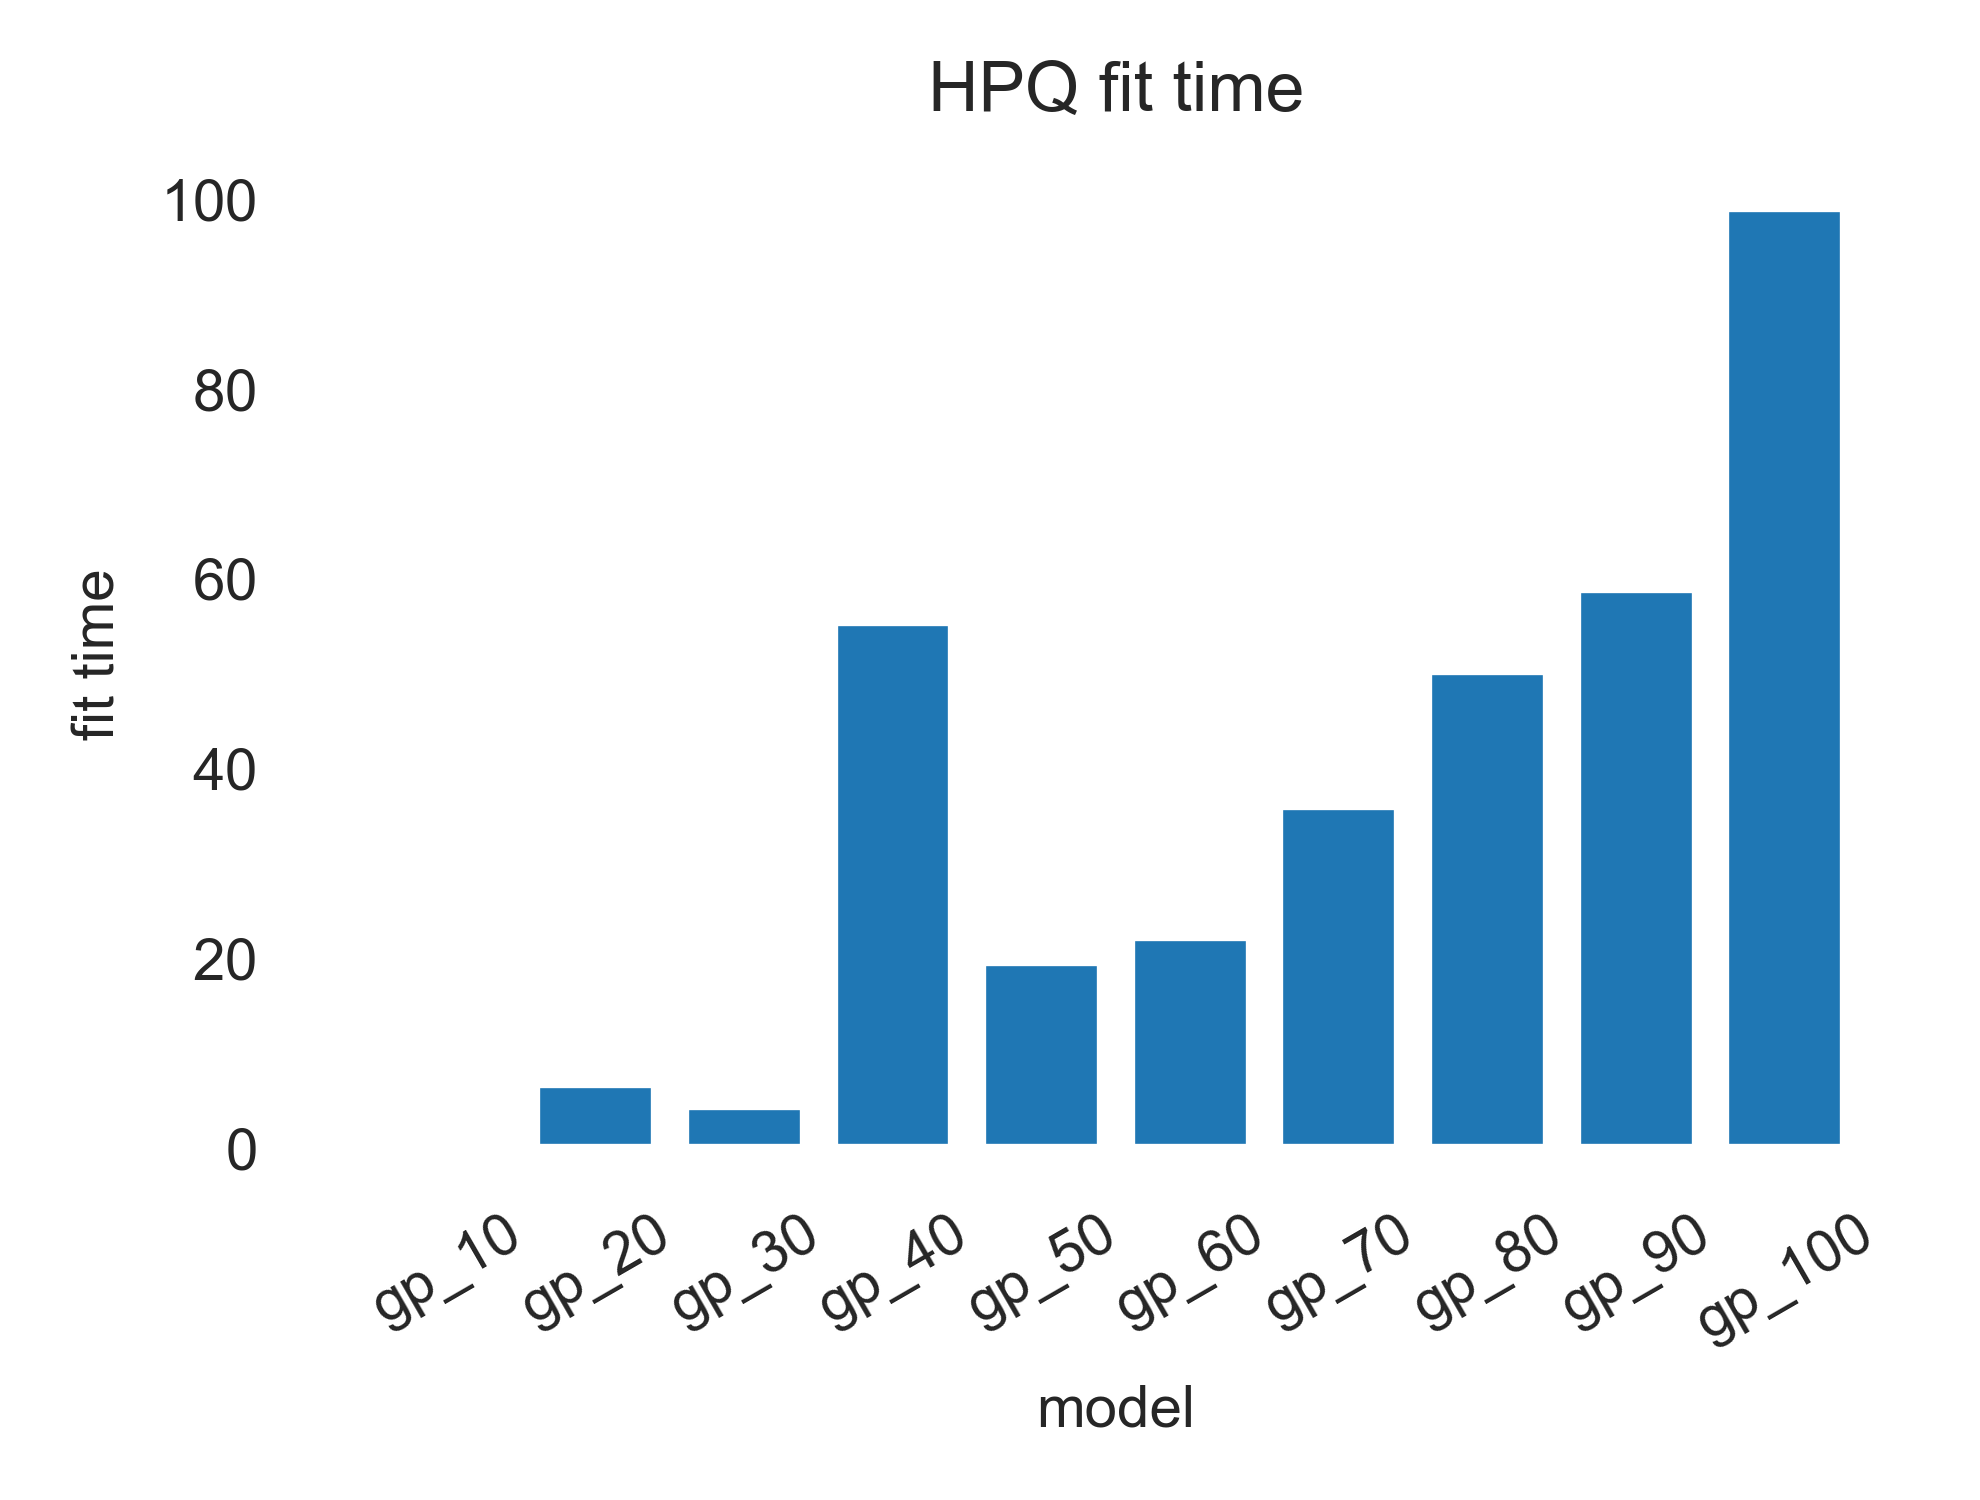
\includegraphics[width=\textwidth]{images/lab2/HPQ_fit_time.png}
    \caption{模型长期预测HPQ时的训练时间}\label{2HPQfittime}
    \end{minipage}
    \begin{minipage}[t]{0.49\textwidth}
    \centering
    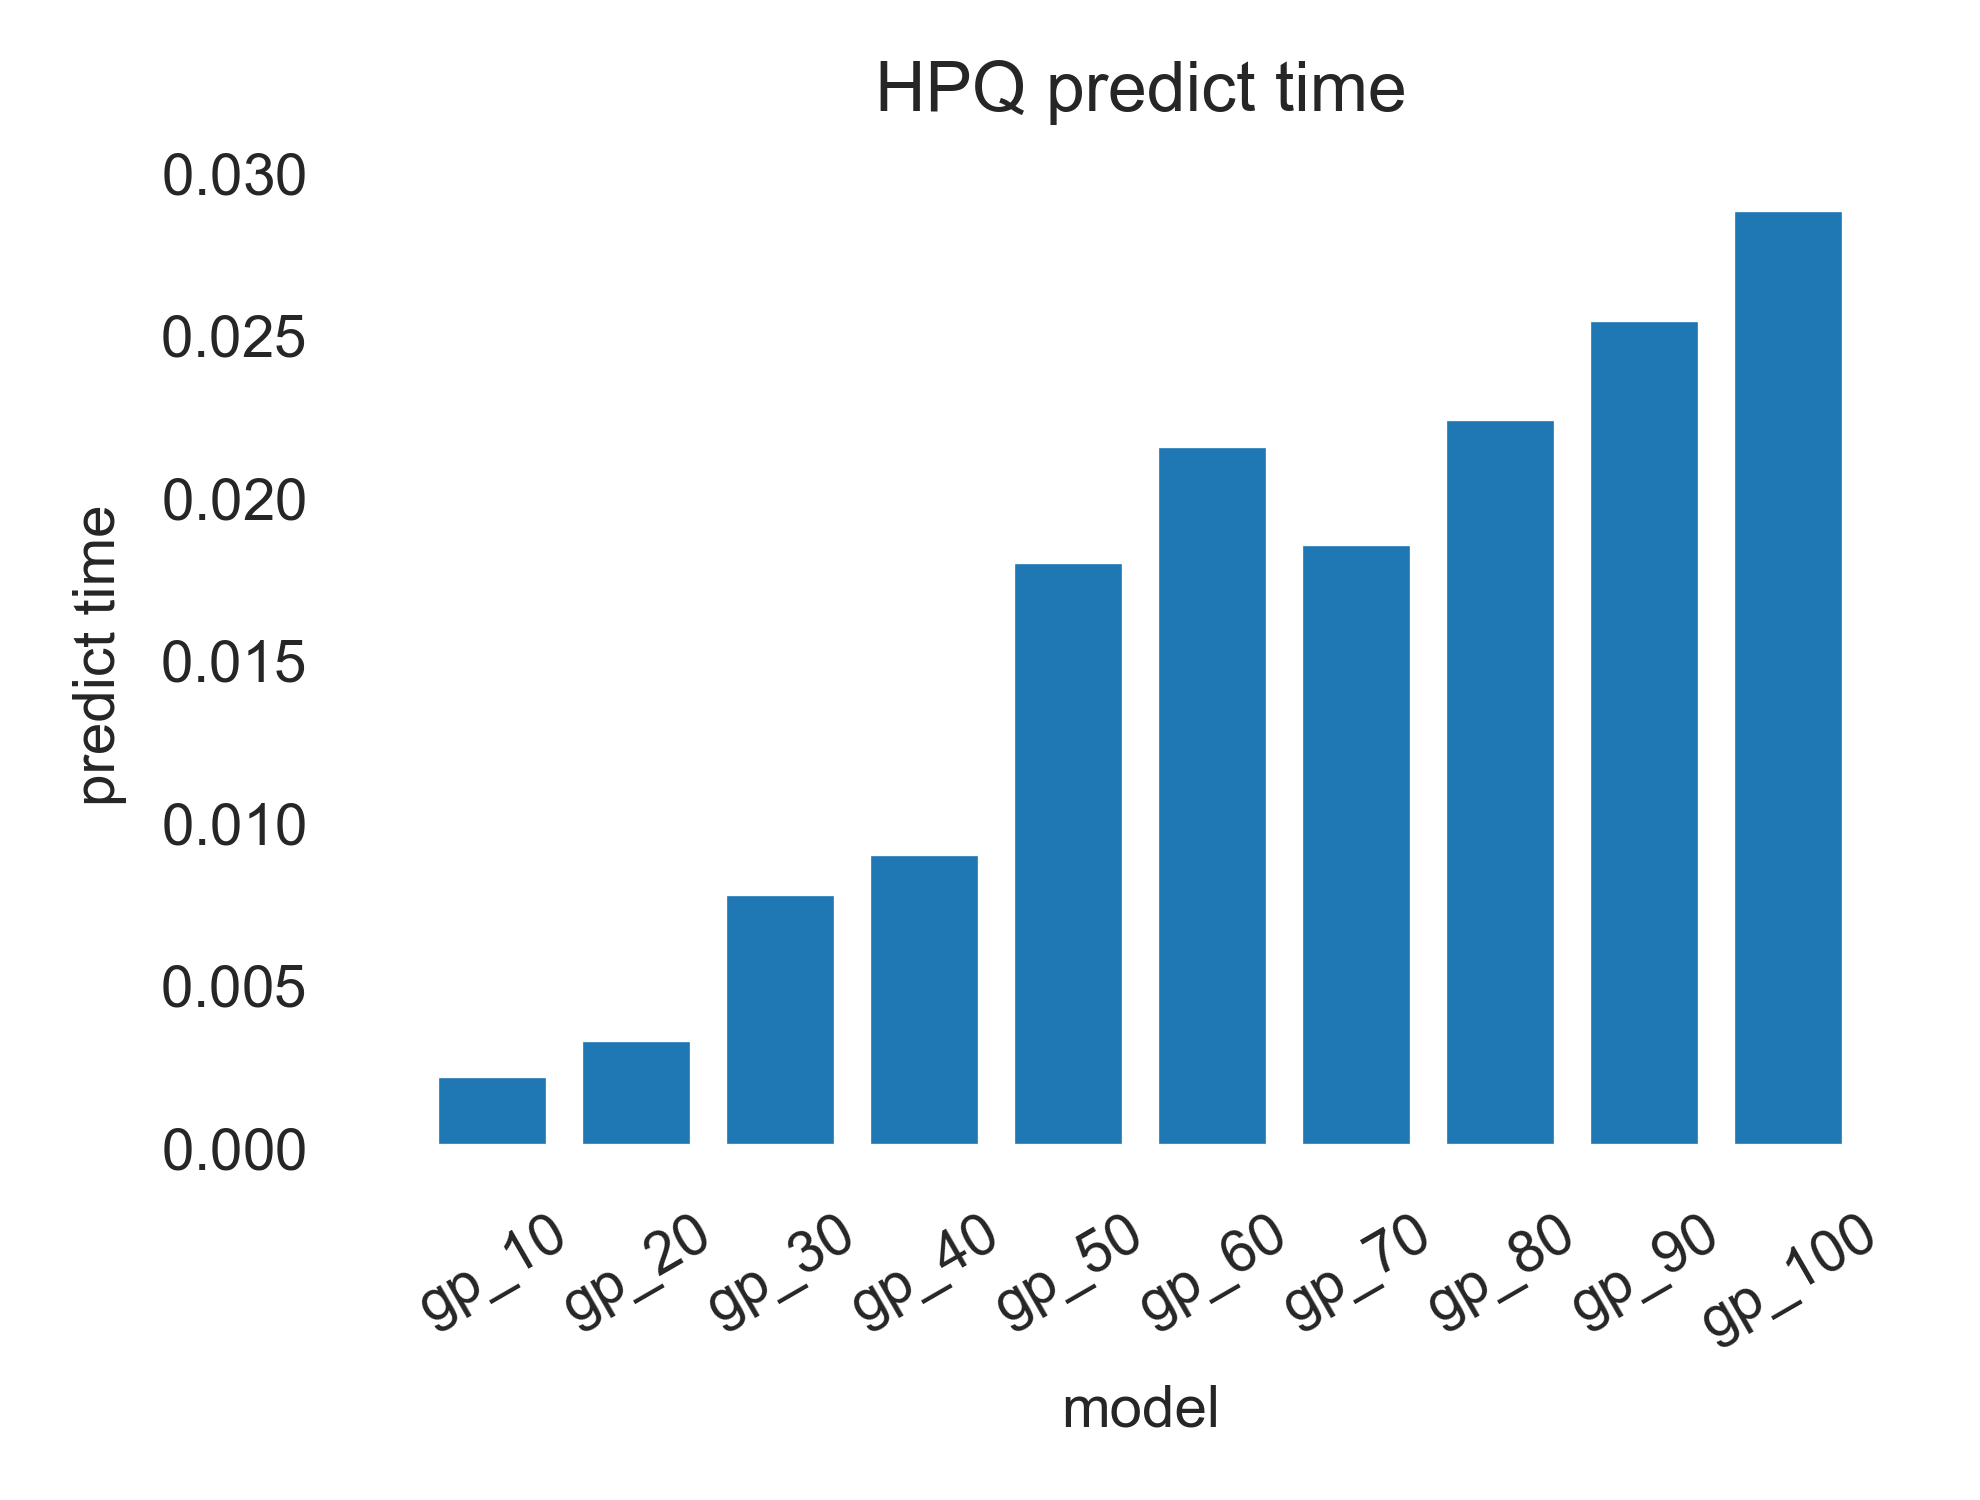
\includegraphics[width=\textwidth]{images/lab2/HPQ_predict_time.png}
    \caption{模型长期预测HPQ时的推理时间}\label{2HPQpredicttime}
    \end{minipage}
\end{figure}

从图\ref{2lab2VZtrend}中可以看出,当使用了超过$50\%$的训练集后,得到的高斯过程模型所给出的长期预测便没有较大的区别。
可能原因是由于后续增加的训练集的样本由距离预测时间段较远的股票价格组成,它们和所预测的股票价格的相关性弱,所以并不会明显影响到
最终的预测结果。

\begin{figure}[!htbp]
    \centering
    \includegraphics[width=\textwidth]{images/lab2/VZ_trend.png}
    \caption{VZ长期趋势}\label{2lab2VZtrend}
\end{figure}

\begin{figure}[!htbp]
    \centering
    \begin{minipage}[t]{0.49\textwidth}
    \centering
    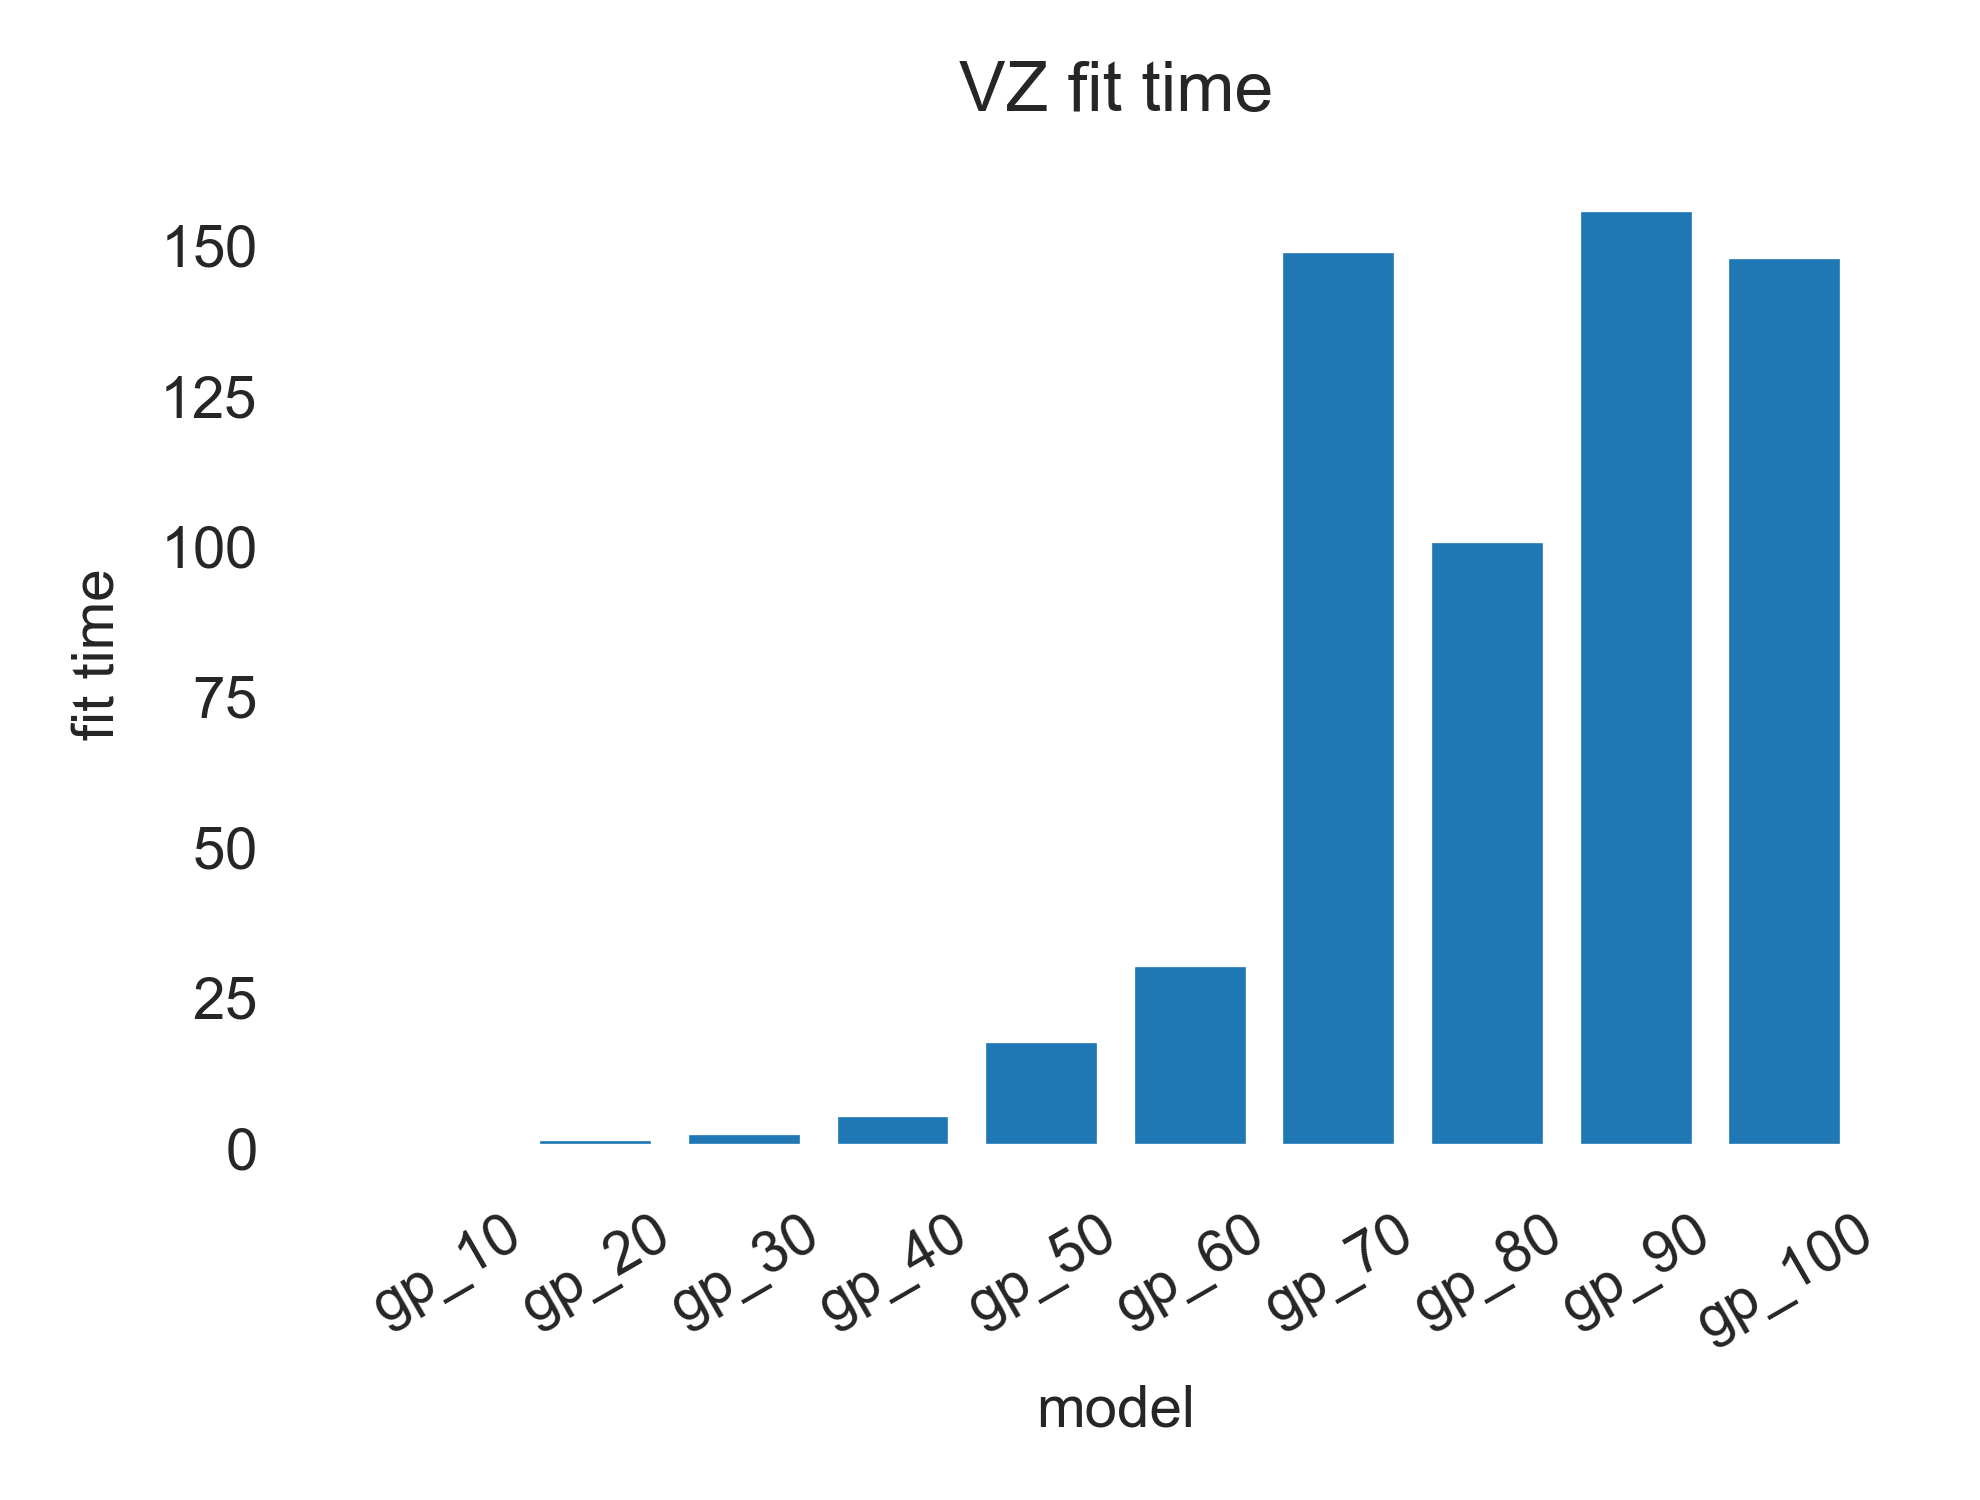
\includegraphics[width=\textwidth]{images/lab2/VZ_fit_time.png}
    \caption{模型长期预测VZ时的训练时间}\label{2VZfittime}
    \end{minipage}
    \begin{minipage}[t]{0.49\textwidth}
    \centering
    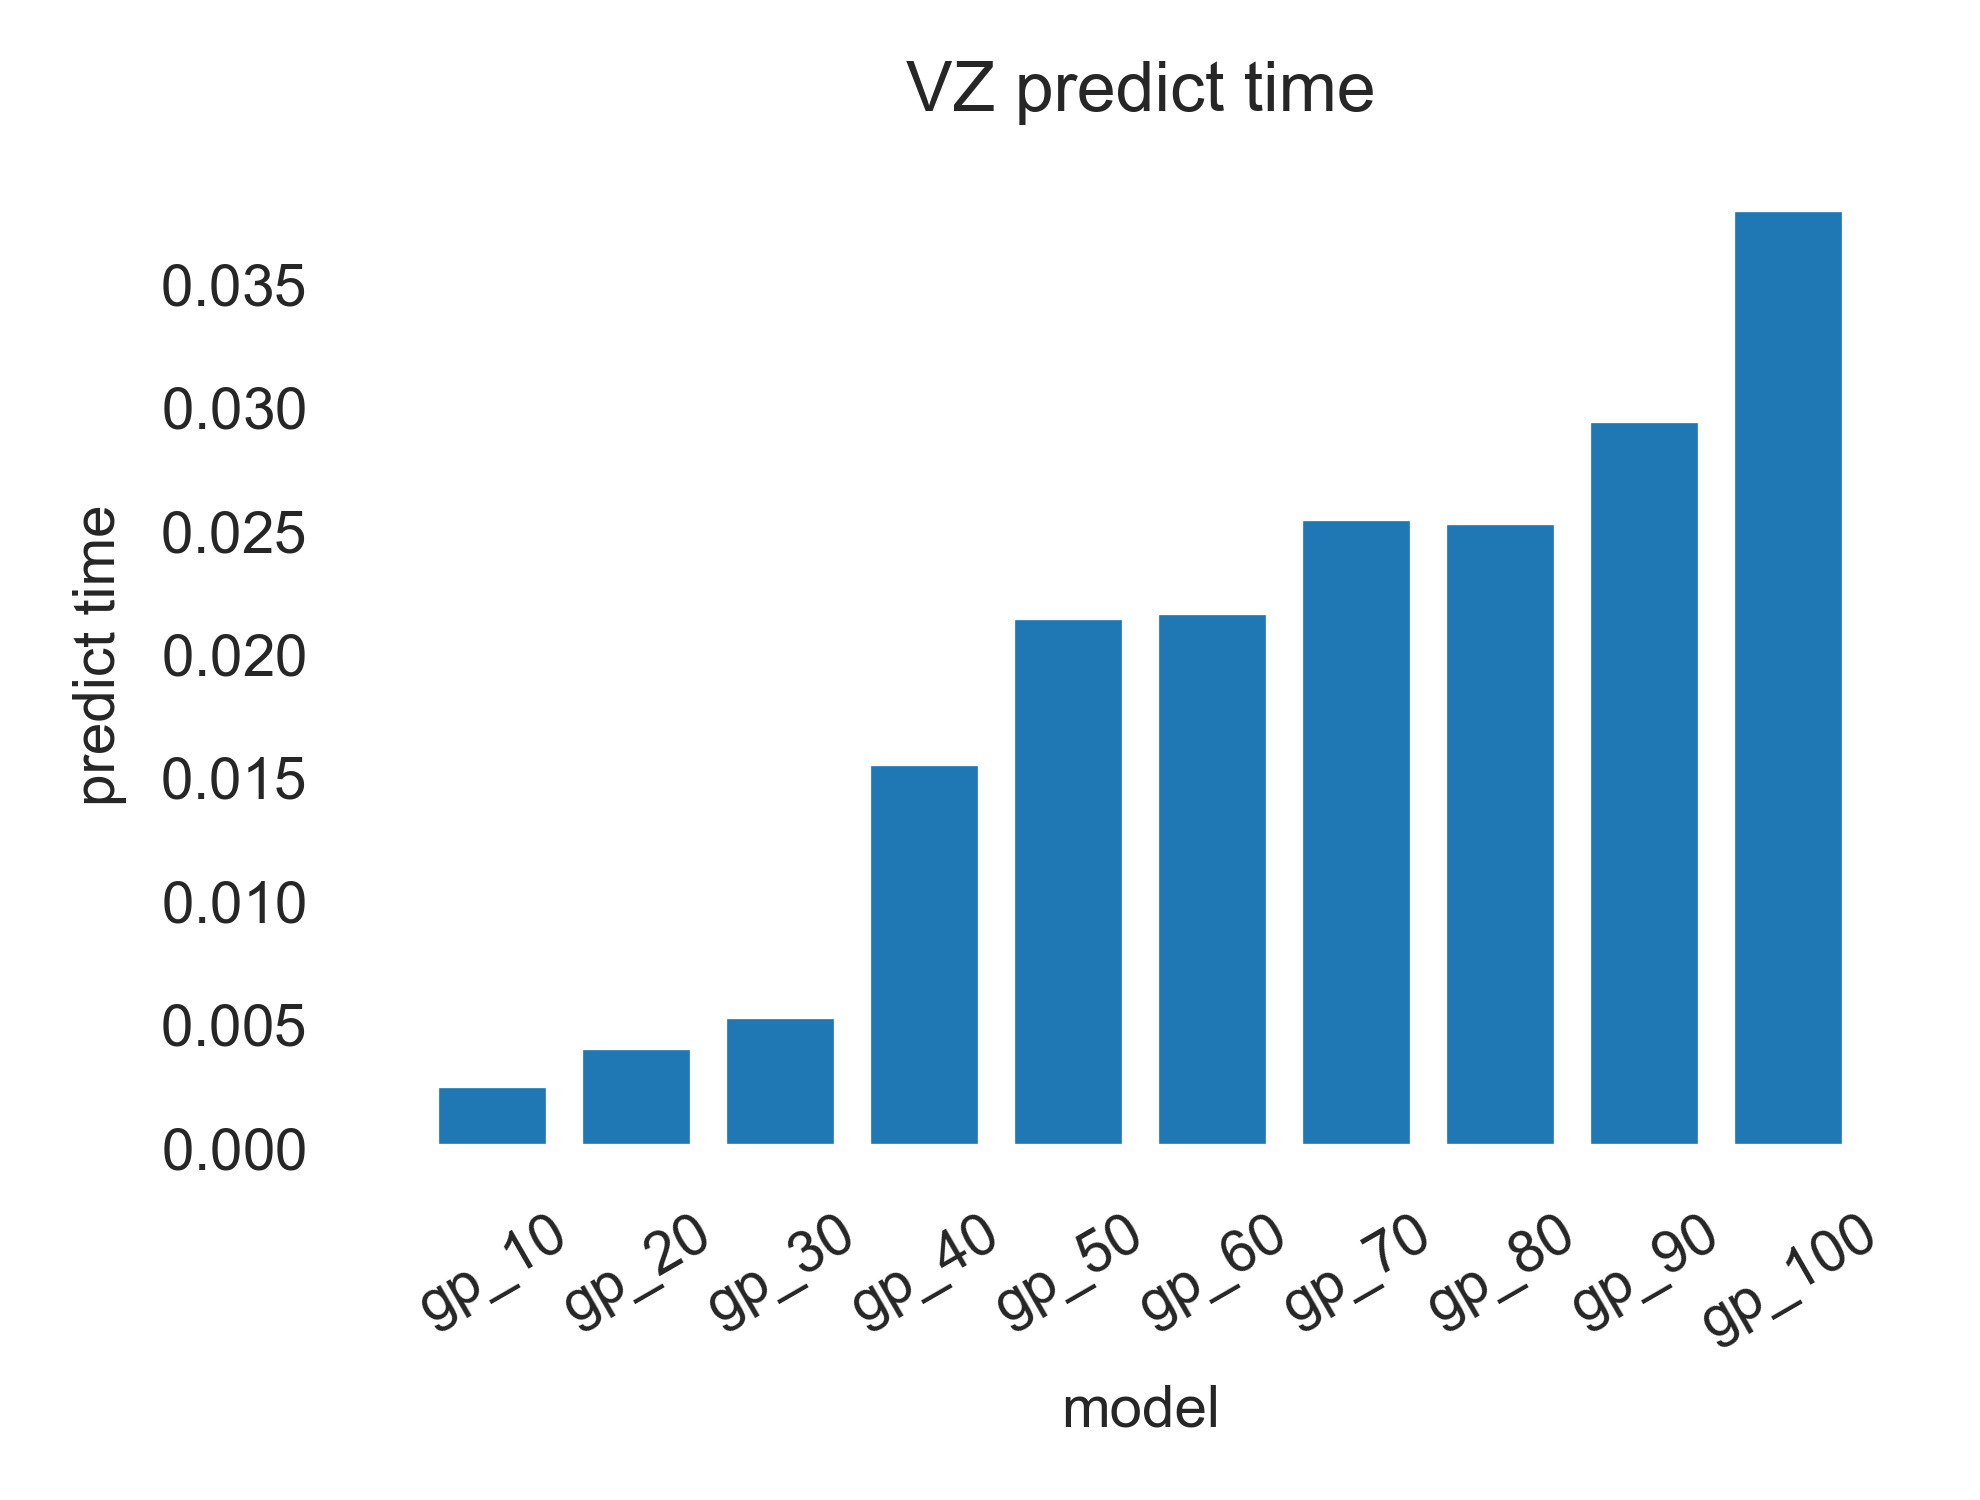
\includegraphics[width=\textwidth]{images/lab2/VZ_predict_time.png}
    \caption{模型长期预测VZ时的推理时间}\label{2VZpredicttime}
    \end{minipage}
\end{figure}

从图\ref{2lab2SBUXtrend}中可以看到,使用$40\%$及以上数据集所得到的高斯过程模型所给出的预测相差不大,它们和
使用较少训练集得到的高斯过程模型$gp\_10$,$gp\_20$,$gp\_30$相比,拐点处和实际股票价格的拐点较为吻合,但同时,依然呈现出快速朝均值衰减的趋势。

\begin{figure}[!htbp]
    \centering
    \includegraphics[width=\textwidth]{images/lab2/SBUX_trend.png}
    \caption{SBUX长期趋势}\label{2lab2SBUXtrend}
\end{figure}


\begin{figure}[!htbp]
    \centering
    \begin{minipage}[t]{0.49\textwidth}
    \centering
    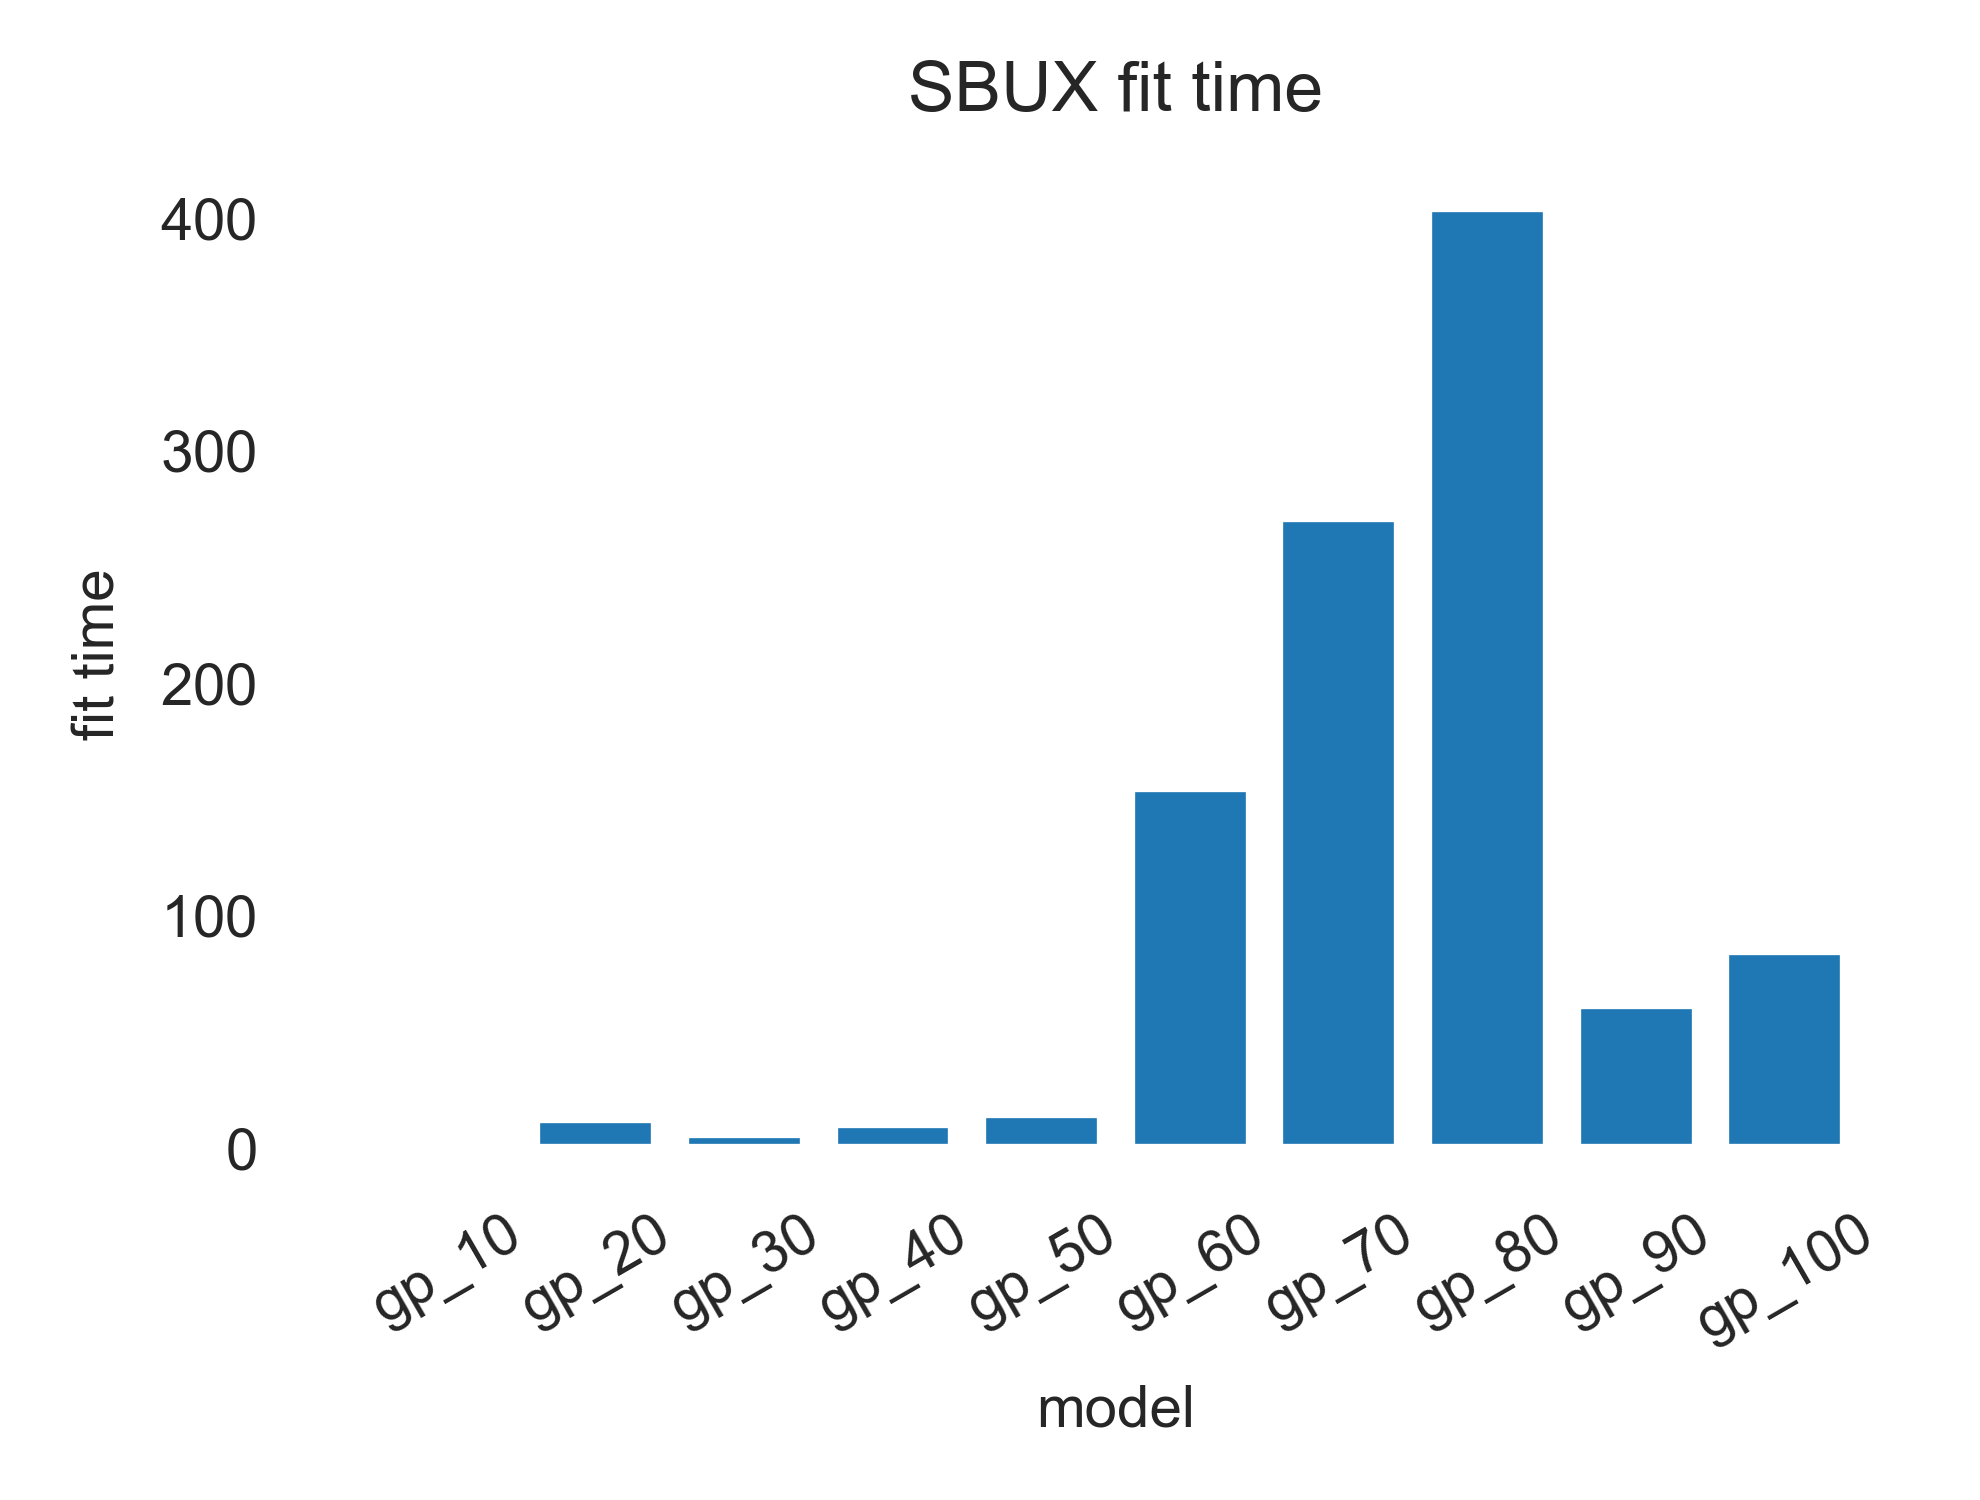
\includegraphics[width=\textwidth]{images/lab2/SBUX_fit_time.png}
    \caption{模型长期预测SBUX时的训练时间}\label{2SBUXfittime}
    \end{minipage}
    \begin{minipage}[t]{0.49\textwidth}
    \centering
    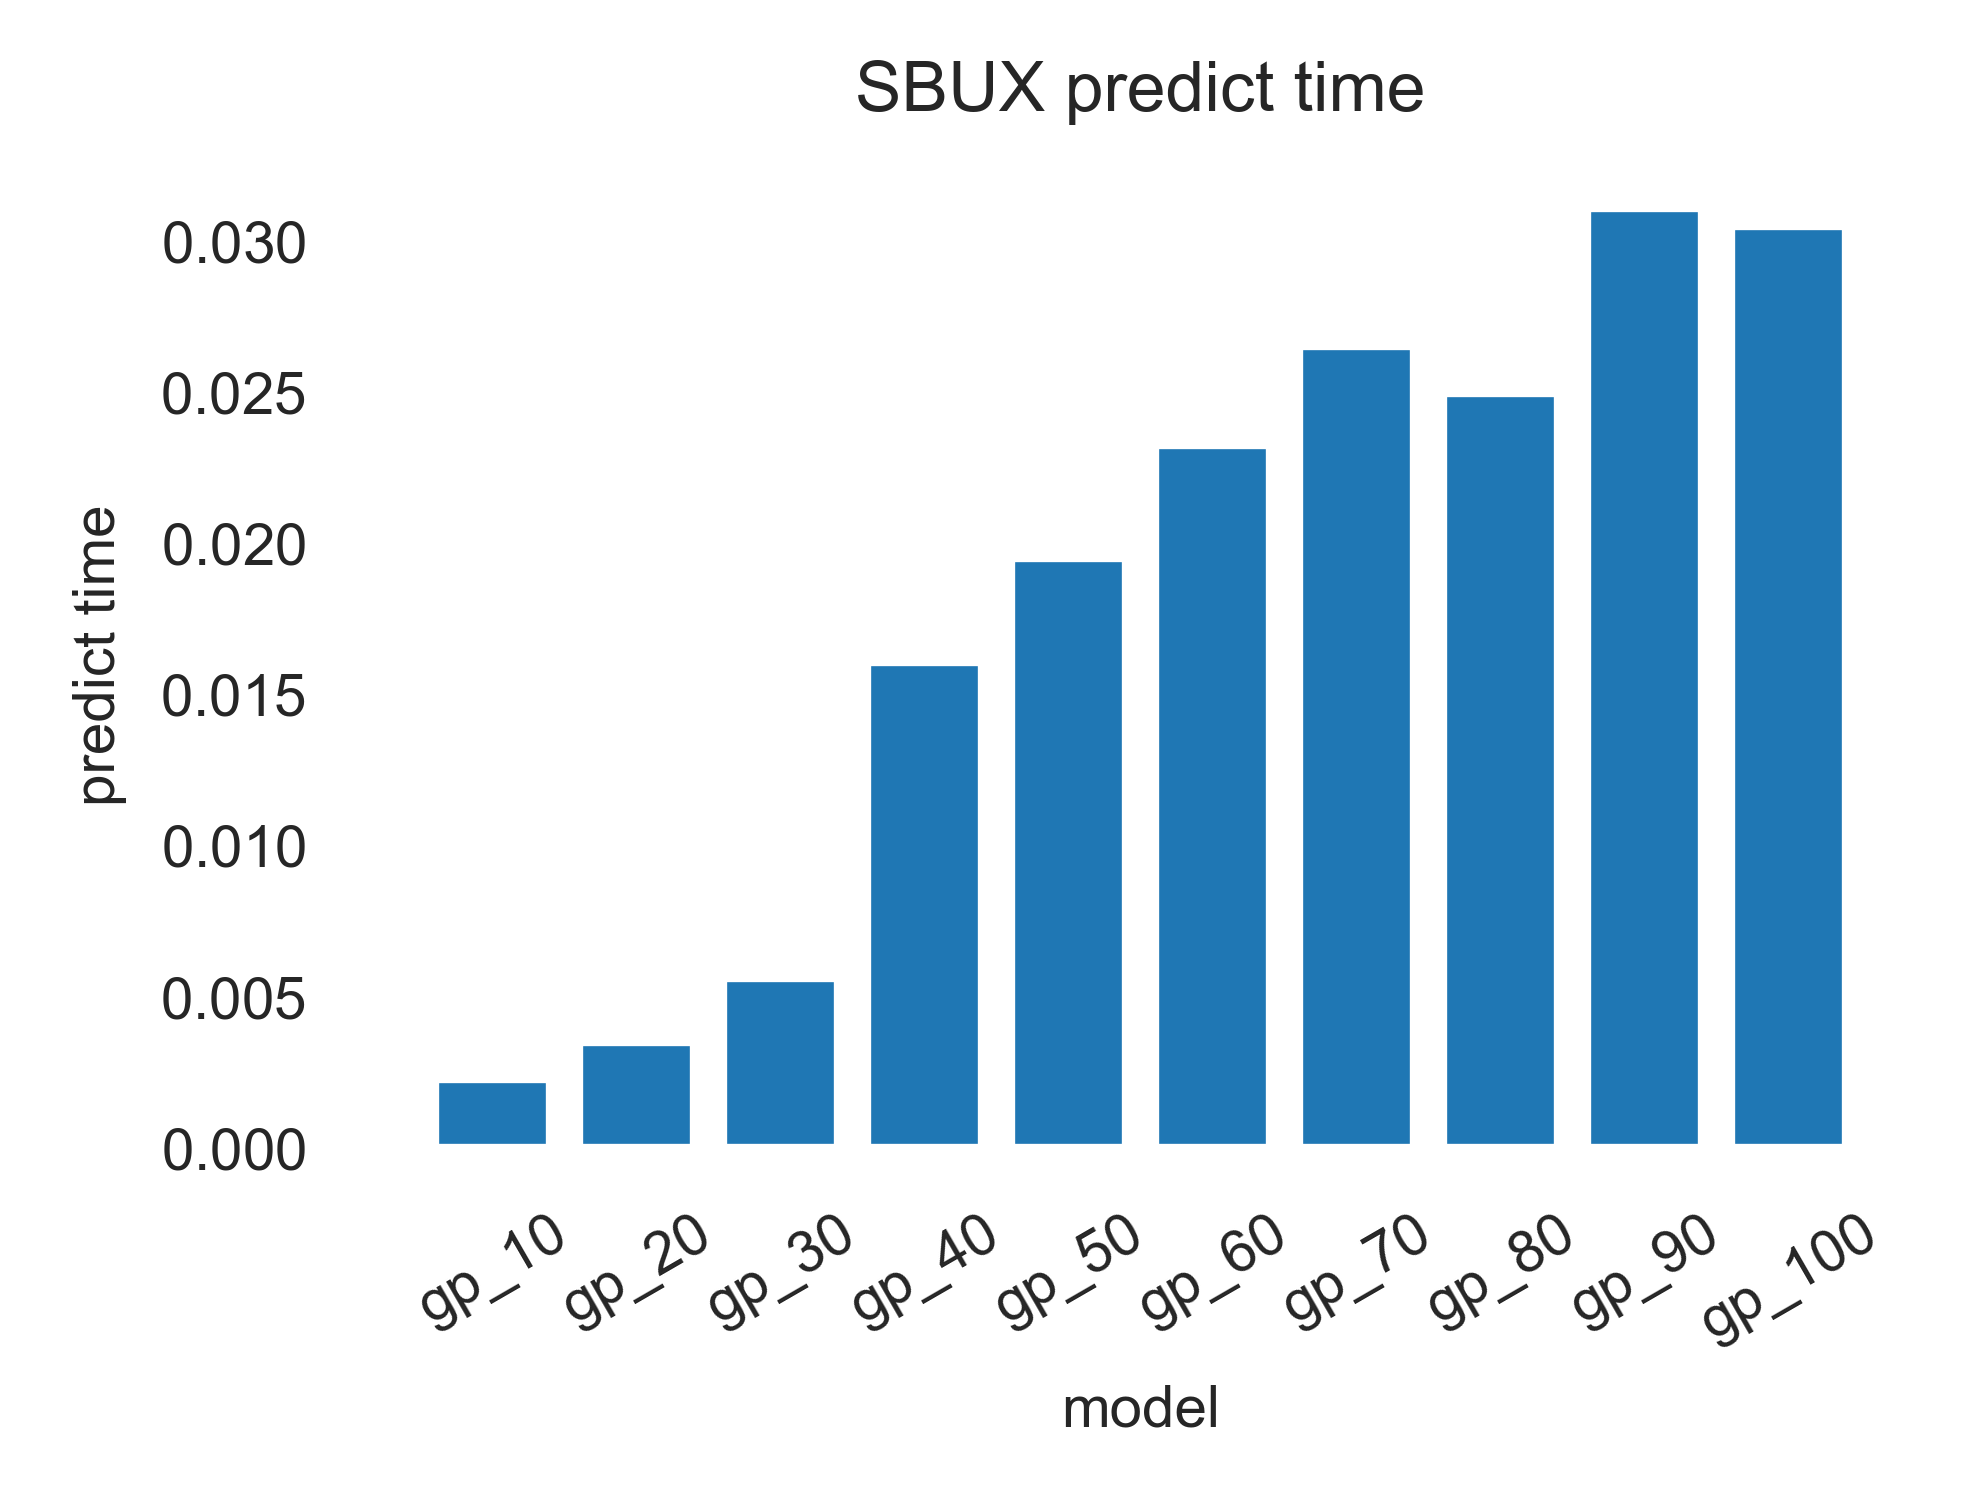
\includegraphics[width=\textwidth]{images/lab2/SBUX_predict_time.png}
    \caption{模型长期预测SBUX时的推理时间}\label{2SBUXpredicttime}
    \end{minipage}
\end{figure}


\subsubsection{高斯过程与稀疏高斯过程在短期预测方面的能力对比}


\begin{figure}[!htbp]
    \centering
    \includegraphics[width=\textwidth]{images/lab3/HPQ_trend.png}
    \caption{HPQ长期趋势}\label{3lab3HPQtrend}
\end{figure}


从图\ref{3lab3HPQtrend}中可以看出,使用完整窗口进行训练的高斯过程模型$gp$,以及使用较多伪数据点的稀疏高斯过程$gp\_30$
所得到的预测结果出现大幅波动的次数较多。但是整体上看,如图\ref{3HPQMAE}所示,这4个模型的MAE差距不大,其中,采用窗口长度的$20\%$作为
伪数据的稀疏高斯过程表现最优。

\begin{figure}[!htbp]
    \centering
    \begin{minipage}[t]{0.49\textwidth}
    \centering
    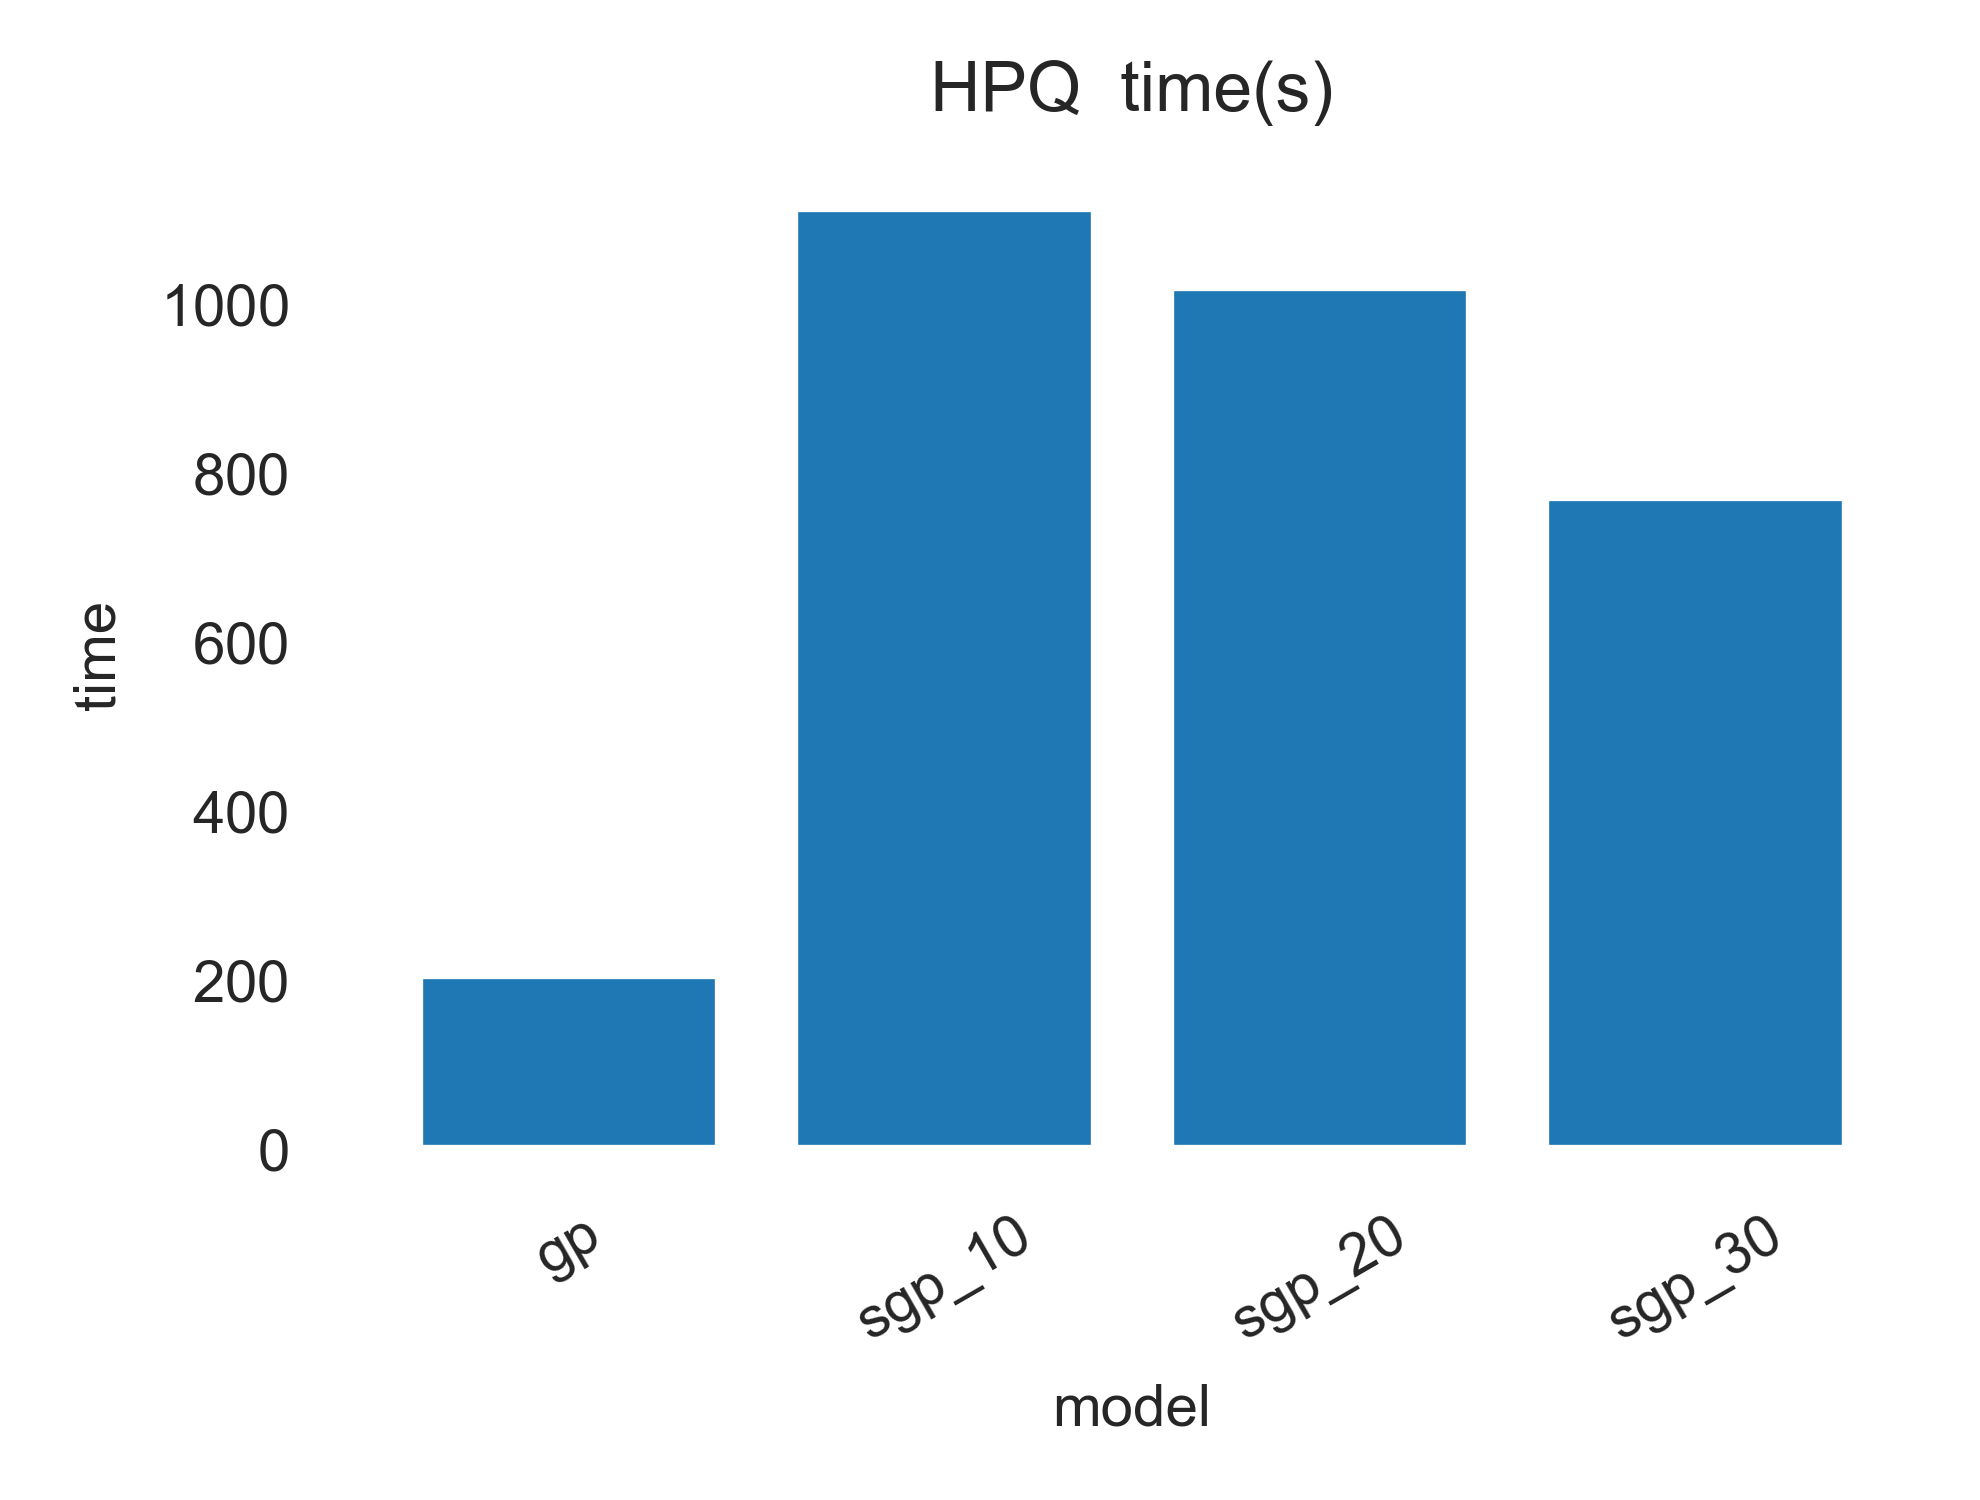
\includegraphics[width=\textwidth]{images/lab3/HPQ_time.png}
    \caption{模型滑动预测HPQ结果的MAE指标}\label{3HPQtime}
    \end{minipage}
    \begin{minipage}[t]{0.49\textwidth}
    \centering
    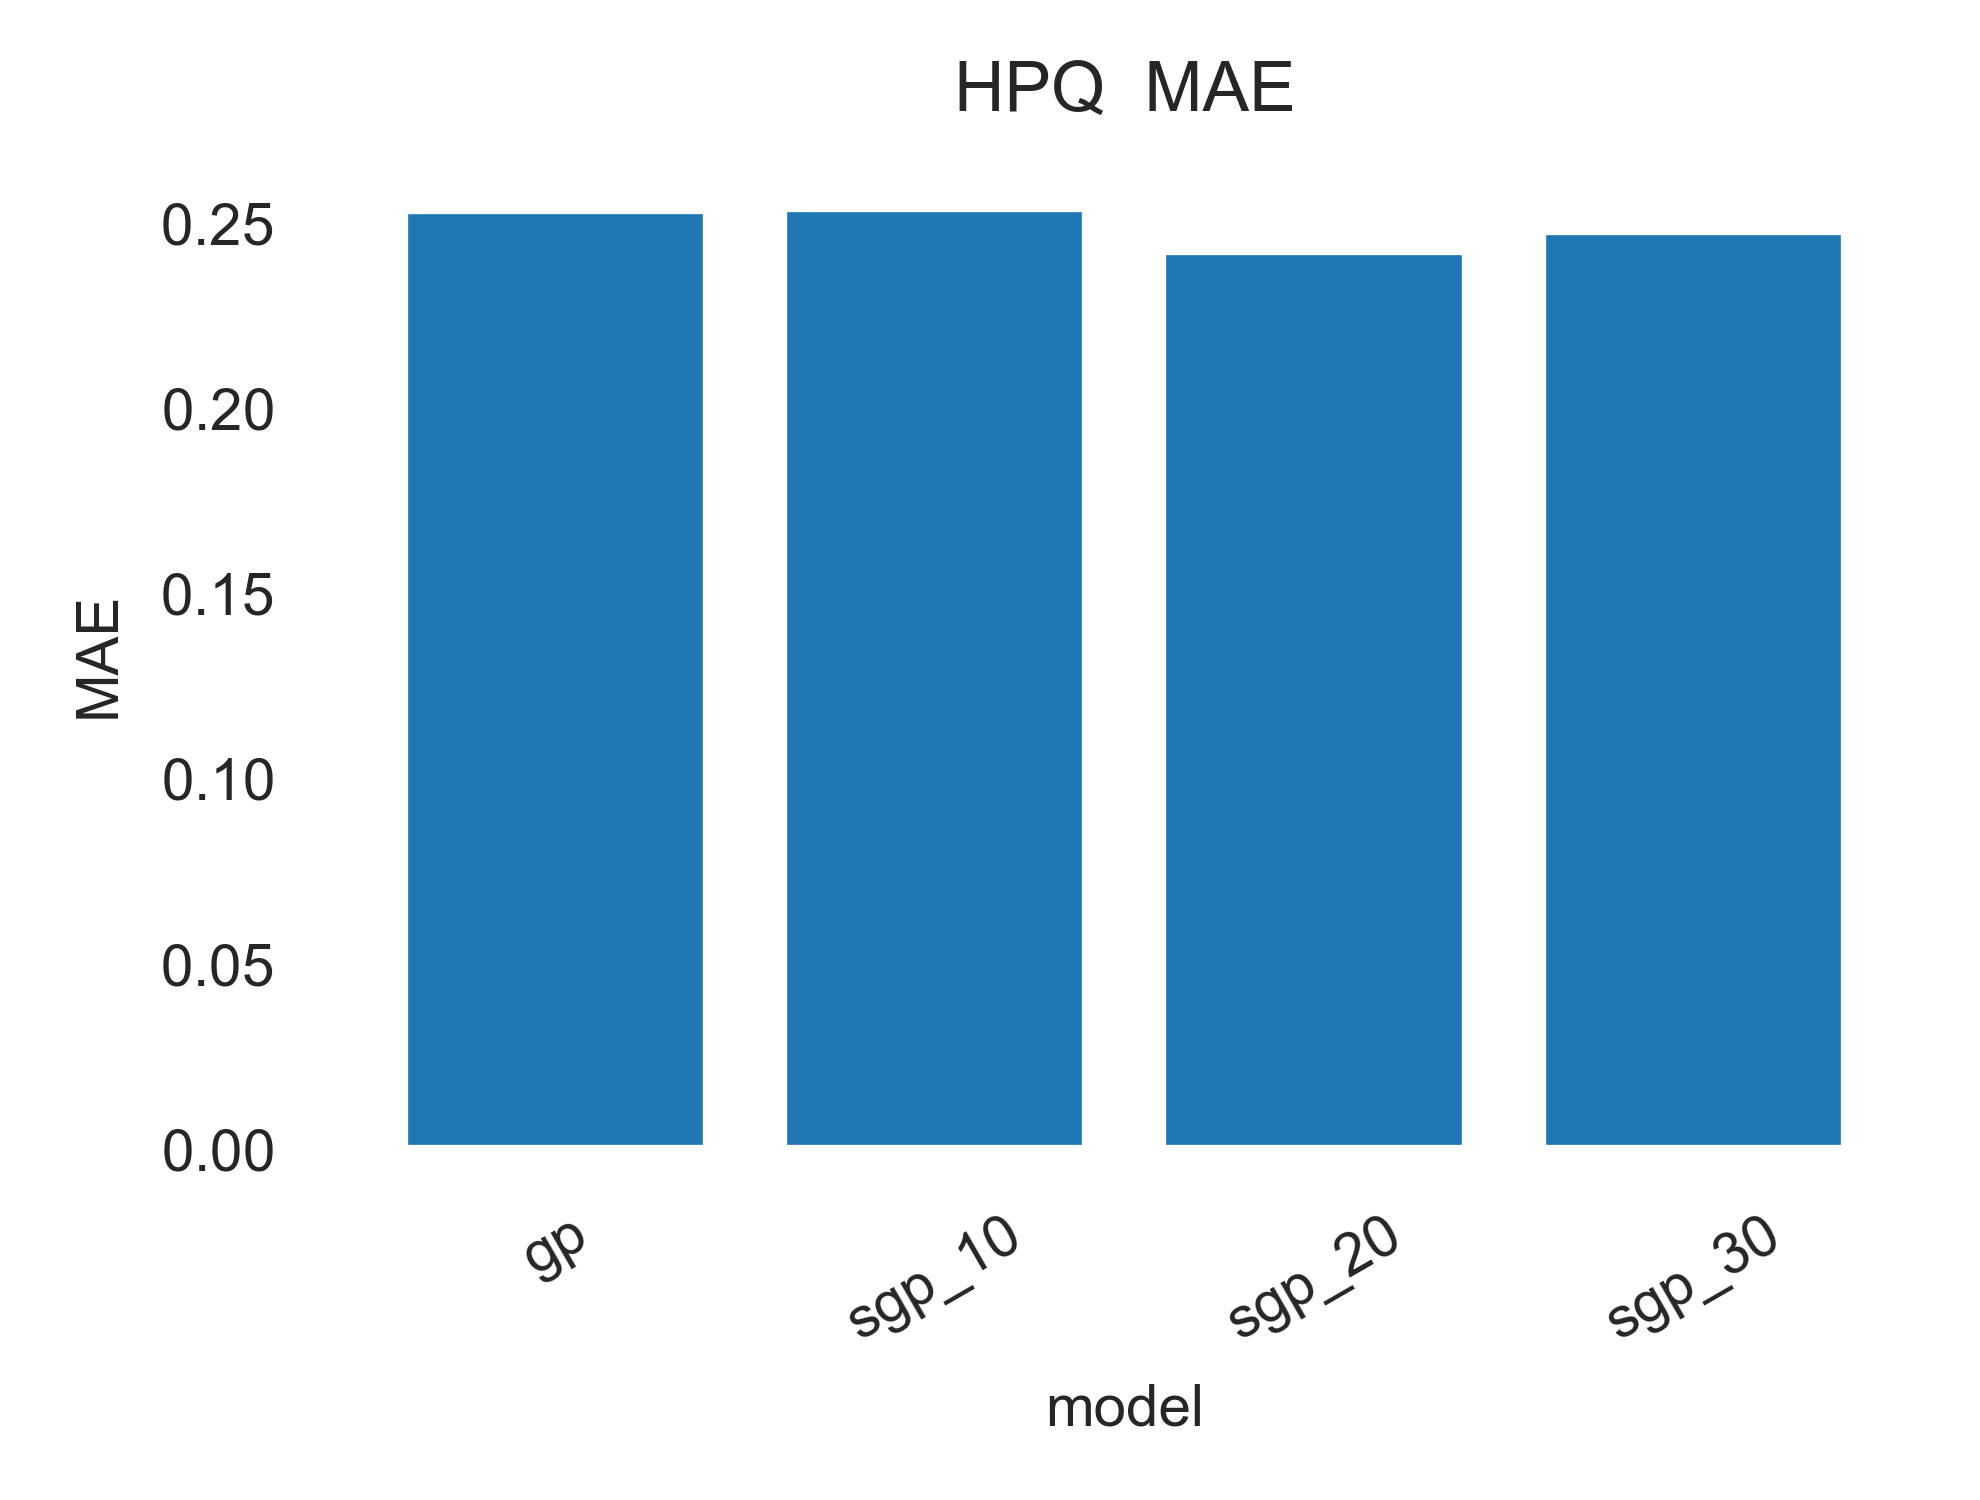
\includegraphics[width=\textwidth]{images/lab3/HPQ_MAE.png}
    \caption{模型滑动预测HPQ时的推理时间}\label{3HPQMAE}
    \end{minipage}
\end{figure}

从预测时间上看,稀疏高斯过程要远高于高斯过程,这一点与我们在进行长期预测时得到的结论不同。
原因在于,在进行长期预测时,每个模型我们只进行一次训练和预测,并且所使用的训练集相较于我们采用的窗口大小,100,较大。
因此,稀疏高斯过程用于调整伪数据点的时间对整体的时间影响较小。而在短期预测时,由于窗口大小较小,导致稀疏高斯过程在时间上的优势不够明显,
加之稀疏高斯过程还需要额外调整伪数据的分布,最终导致了稀疏高斯过程所消耗的时间是高斯过程的数倍。

值得注意的时,在短期预测时,采用较多伪数据的高斯过程所需的训练时间反而会减少,其可能原因在于当伪数据点较多时,可以调整的空间较少,
从而稀疏高斯过程中用于调整伪数据的时间较少。

\begin{figure}[!htbp]
    \centering
    \includegraphics[width=\textwidth]{images/lab3/VZ_trend.png}
    \caption{VZ长期趋势}\label{3lab3VZtrend}
\end{figure}

\begin{figure}[!htbp]
    \centering
    \begin{minipage}[t]{0.49\textwidth}
    \centering
    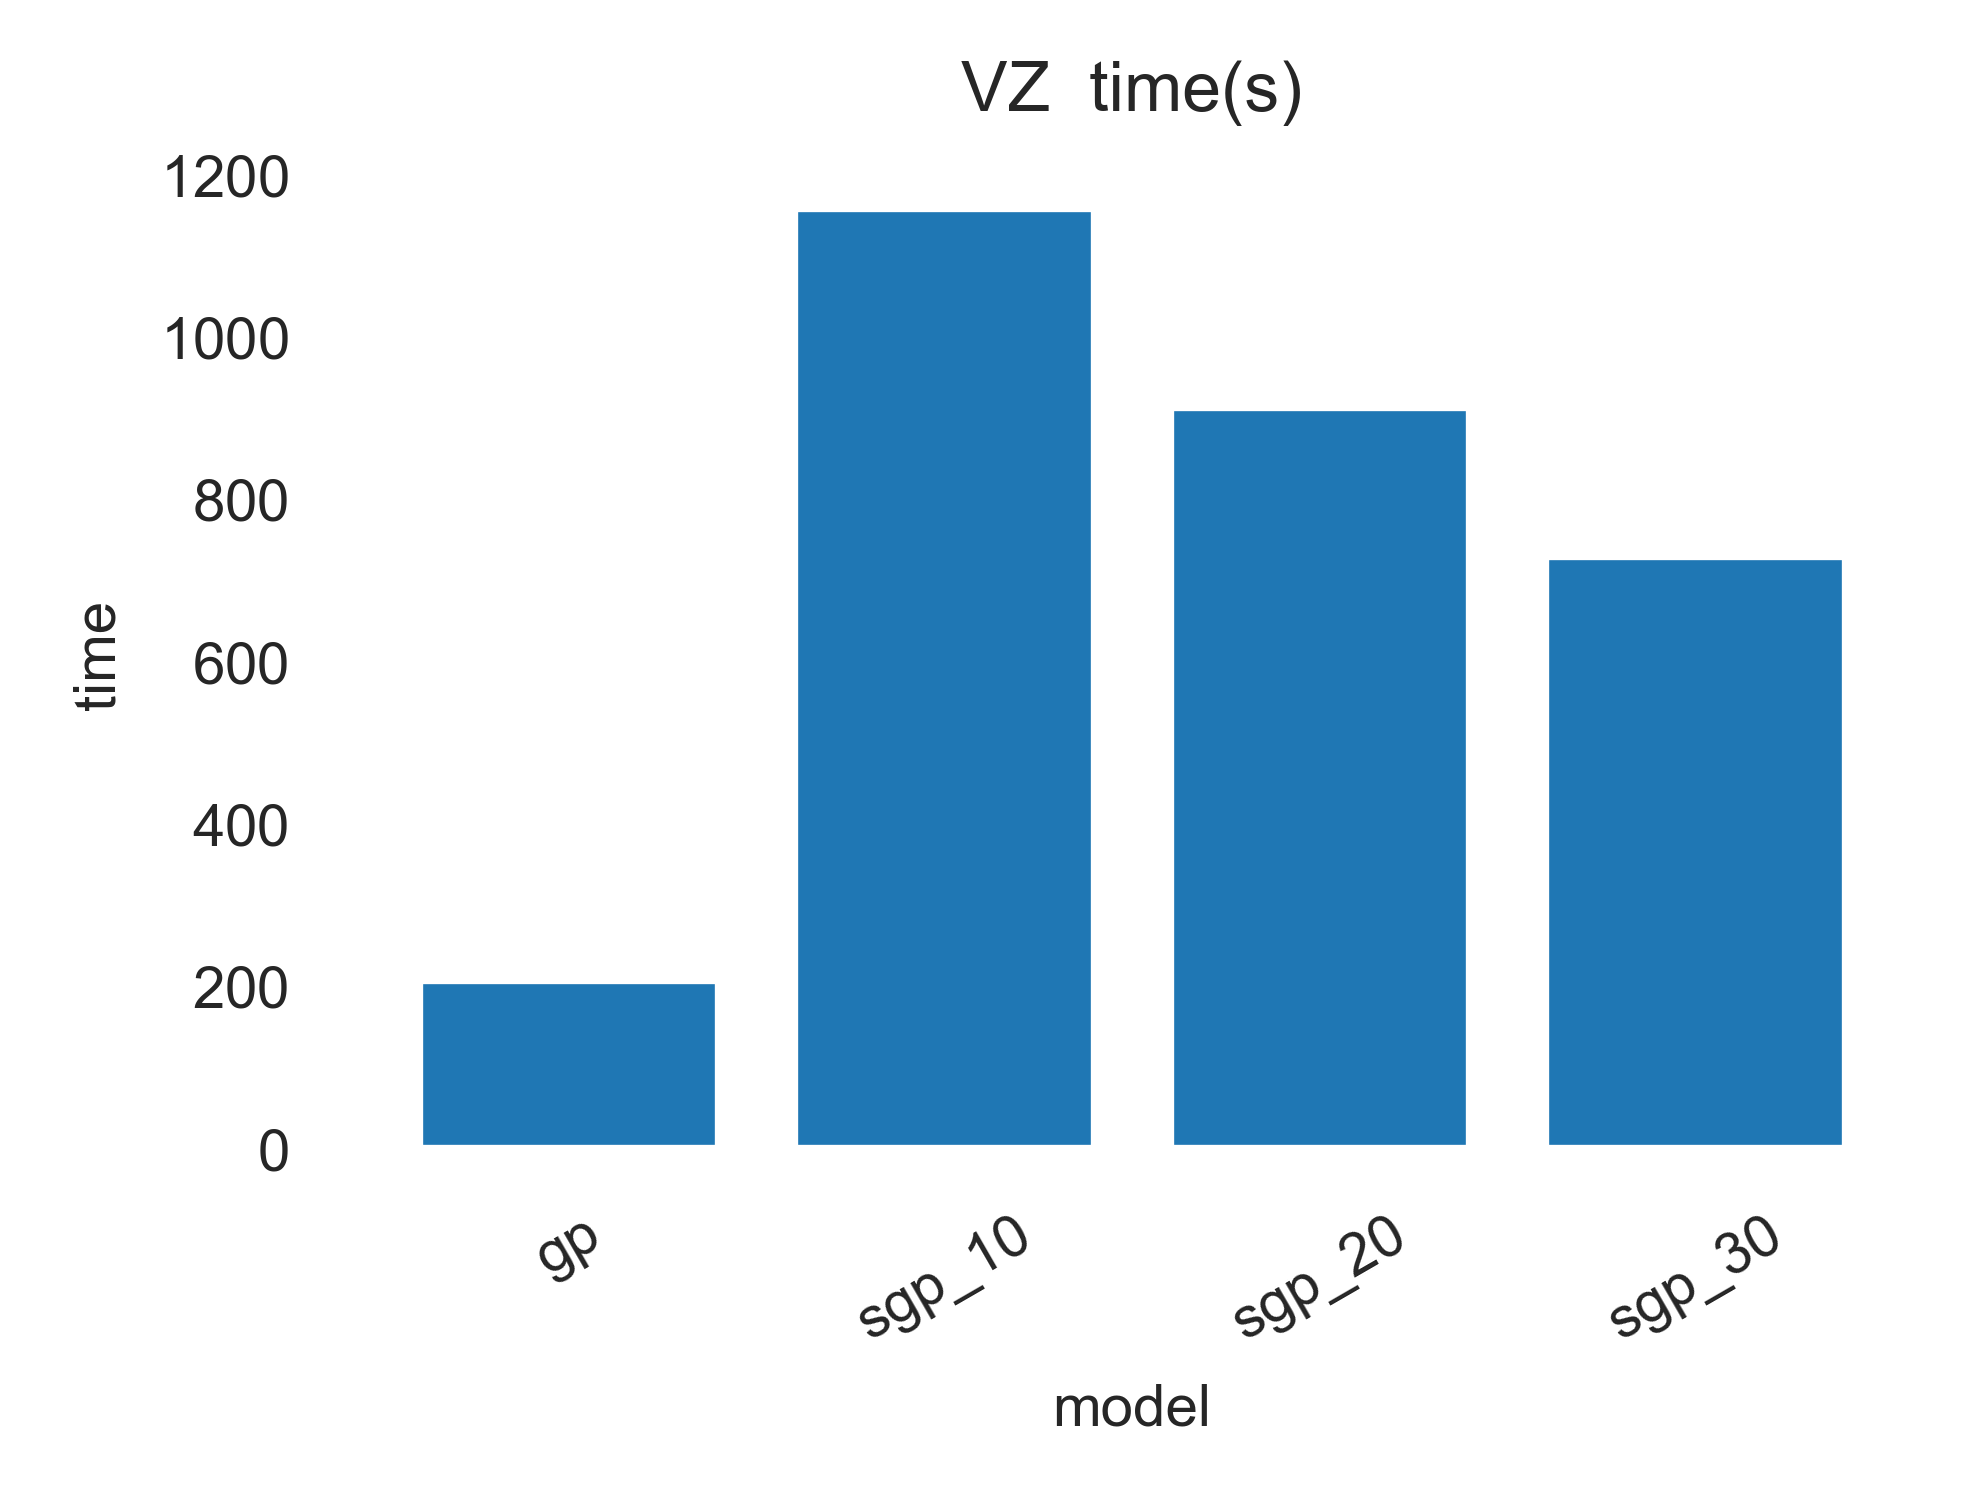
\includegraphics[width=\textwidth]{images/lab3/VZ_time.png}
    \caption{模型滑动预测VZ结果的MAE指标}\label{3VZtime}
    \end{minipage}
    \begin{minipage}[t]{0.49\textwidth}
    \centering
    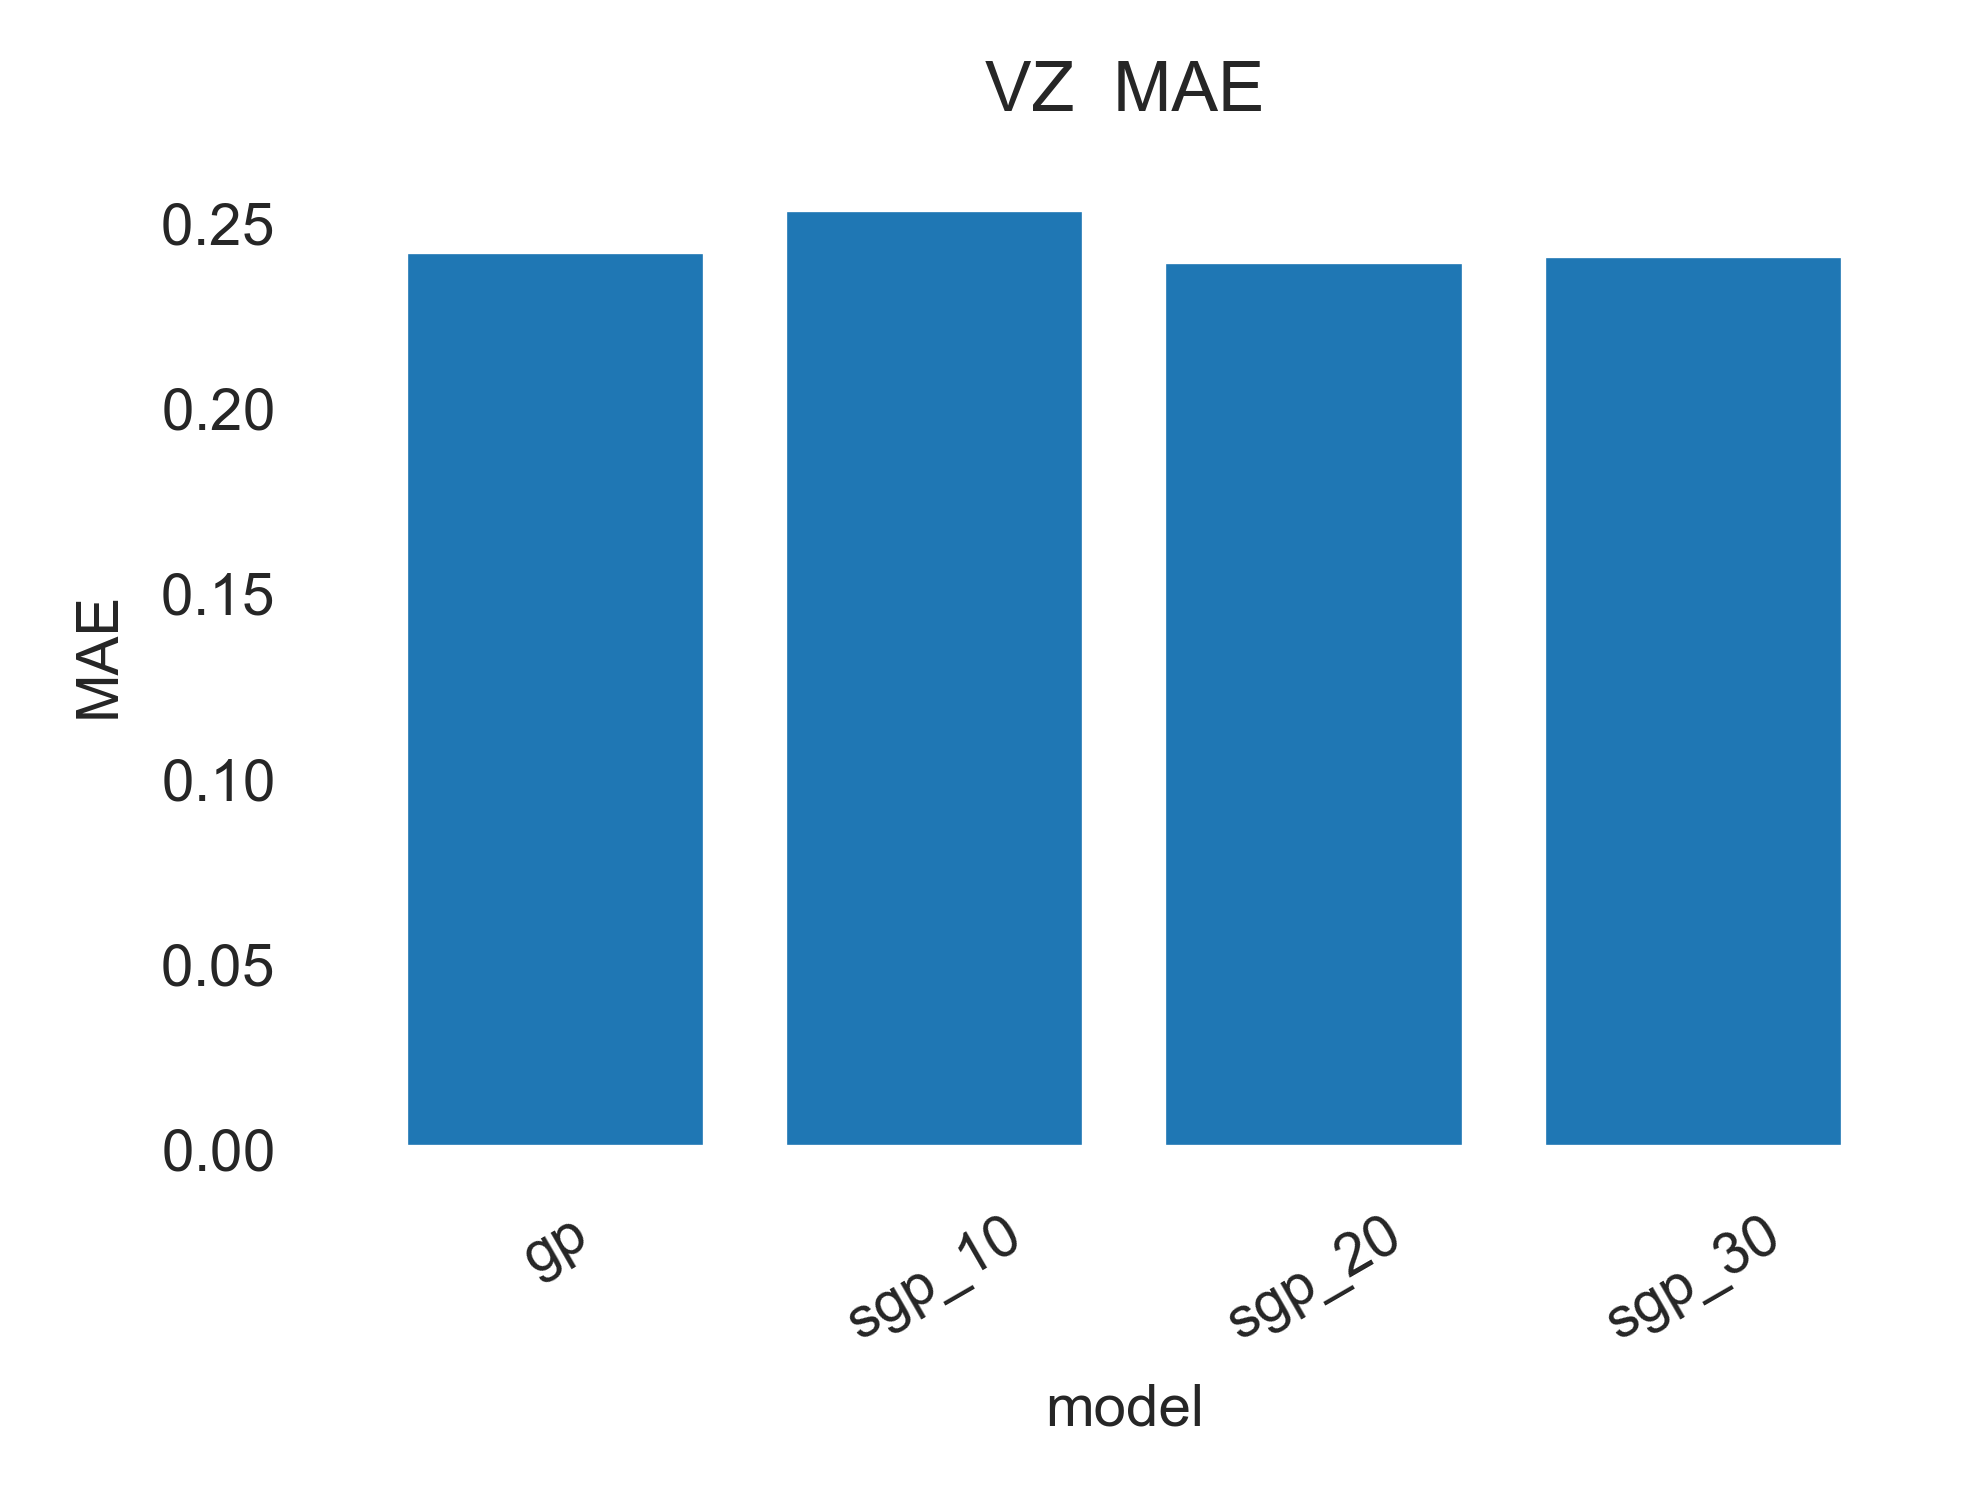
\includegraphics[width=\textwidth]{images/lab3/VZ_MAE.png}
    \caption{模型滑动预测VZ时的推理时间}\label{3VZMAE}
    \end{minipage}
\end{figure}

\begin{figure}[!htbp]
    \centering
    \includegraphics[width=\textwidth]{images/lab3/SBUX_trend.png}
    \caption{SBUX长期趋势}\label{3lab3SBUXtrend}
\end{figure}


\begin{figure}[!htbp]
    \centering
    \begin{minipage}[t]{0.49\textwidth}
    \centering
    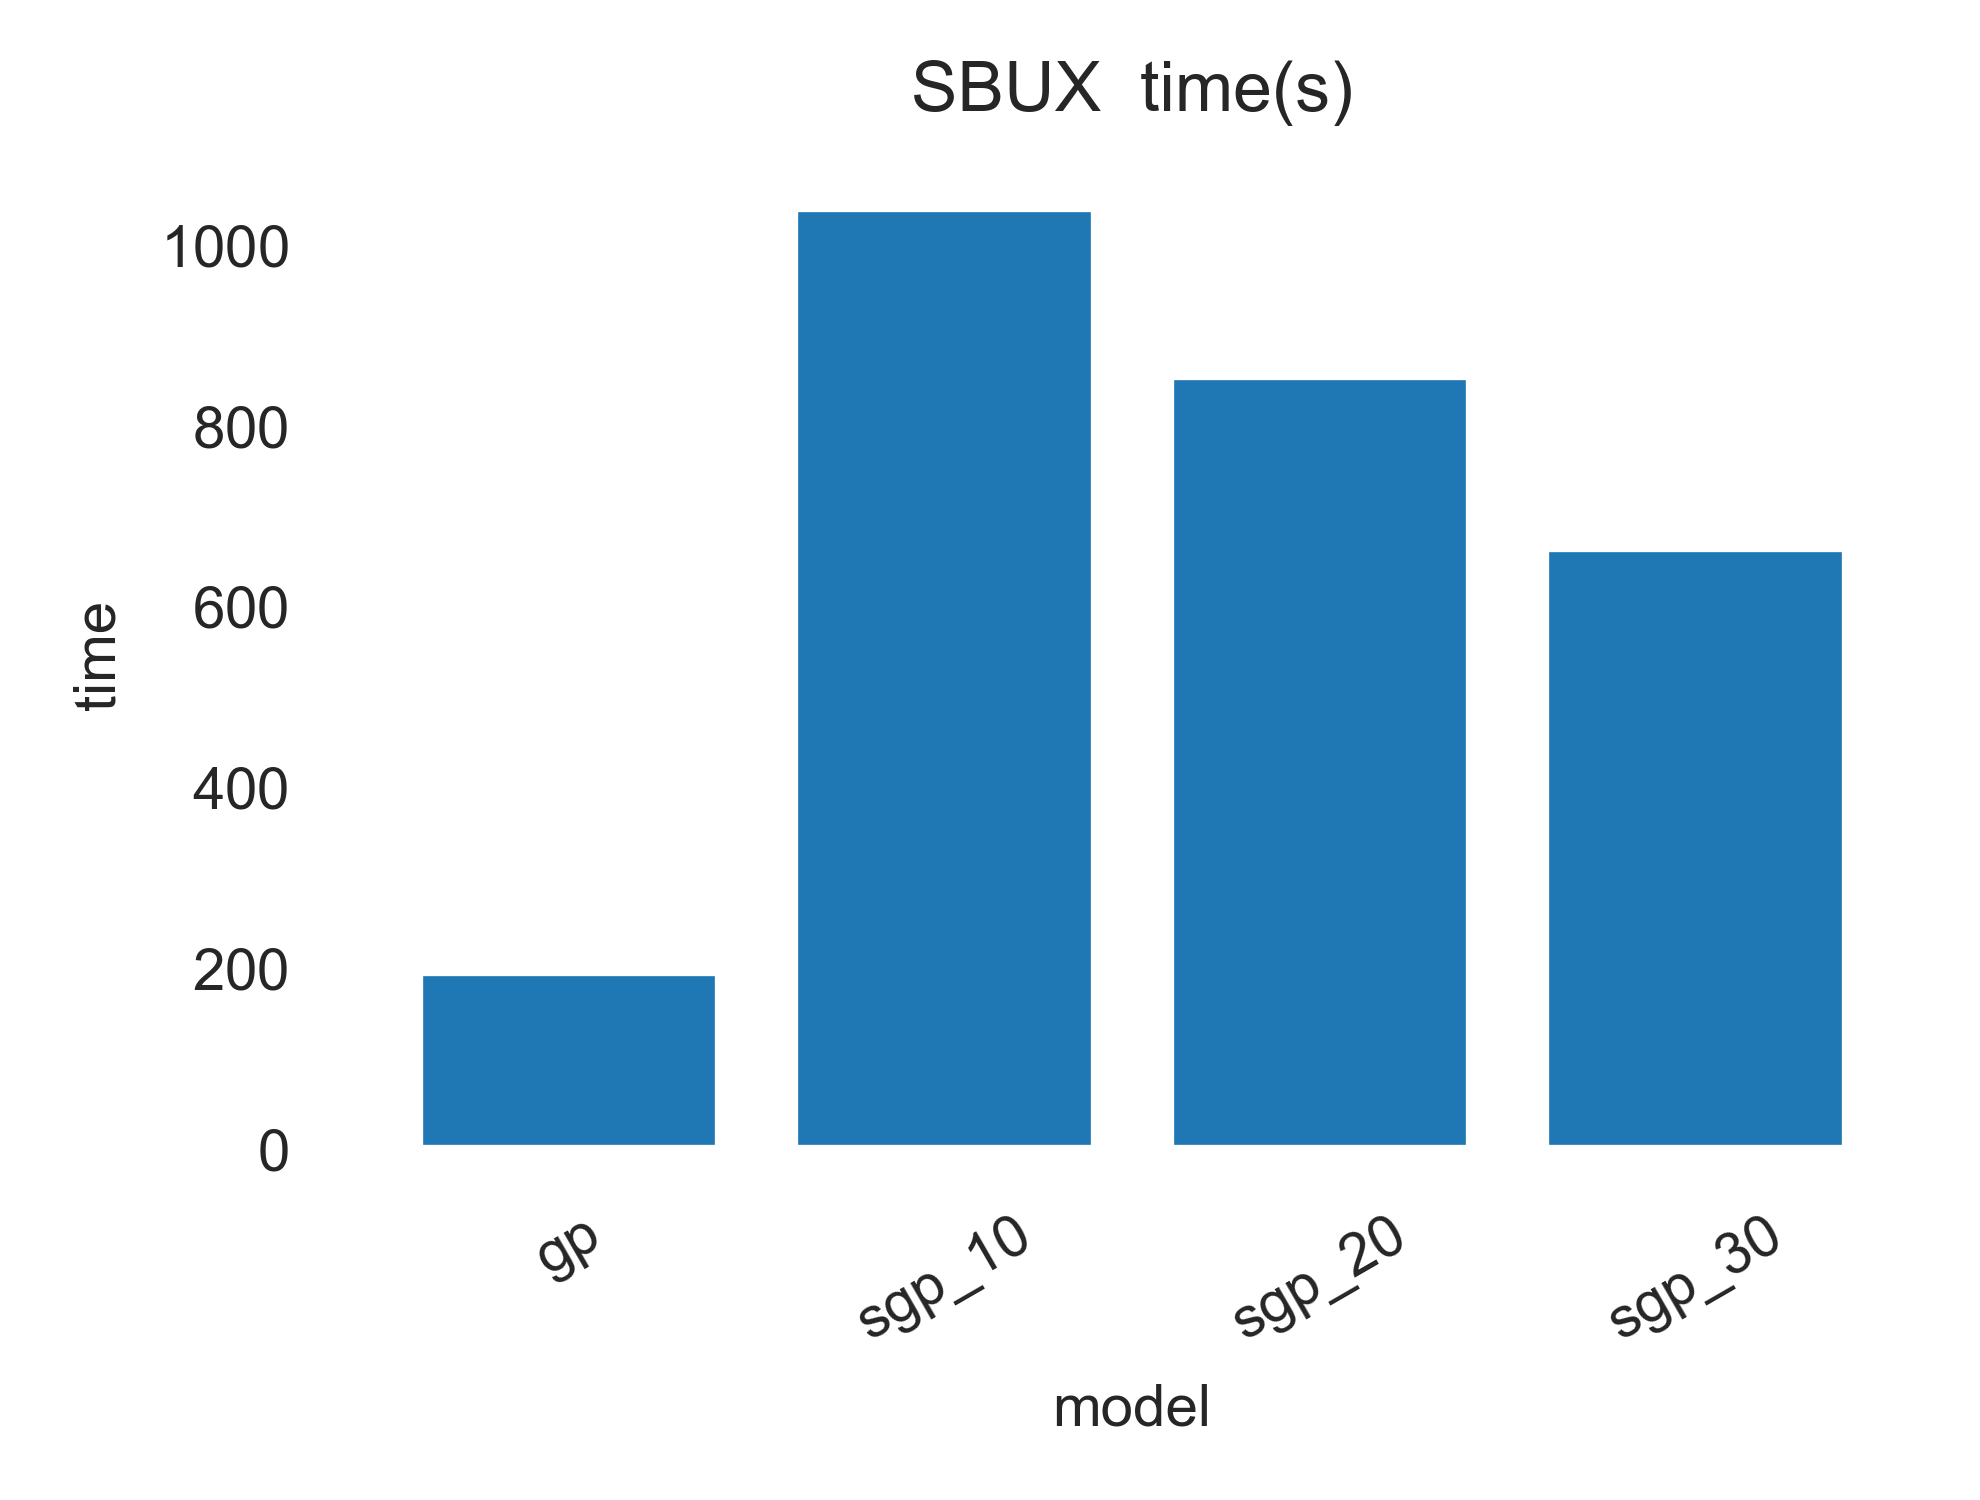
\includegraphics[width=\textwidth]{images/lab3/SBUX_time.png}
    \caption{模型滑动预测SBUX结果的MAE指标}\label{3SBUXtime}
    \end{minipage}
    \begin{minipage}[t]{0.49\textwidth}
    \centering
    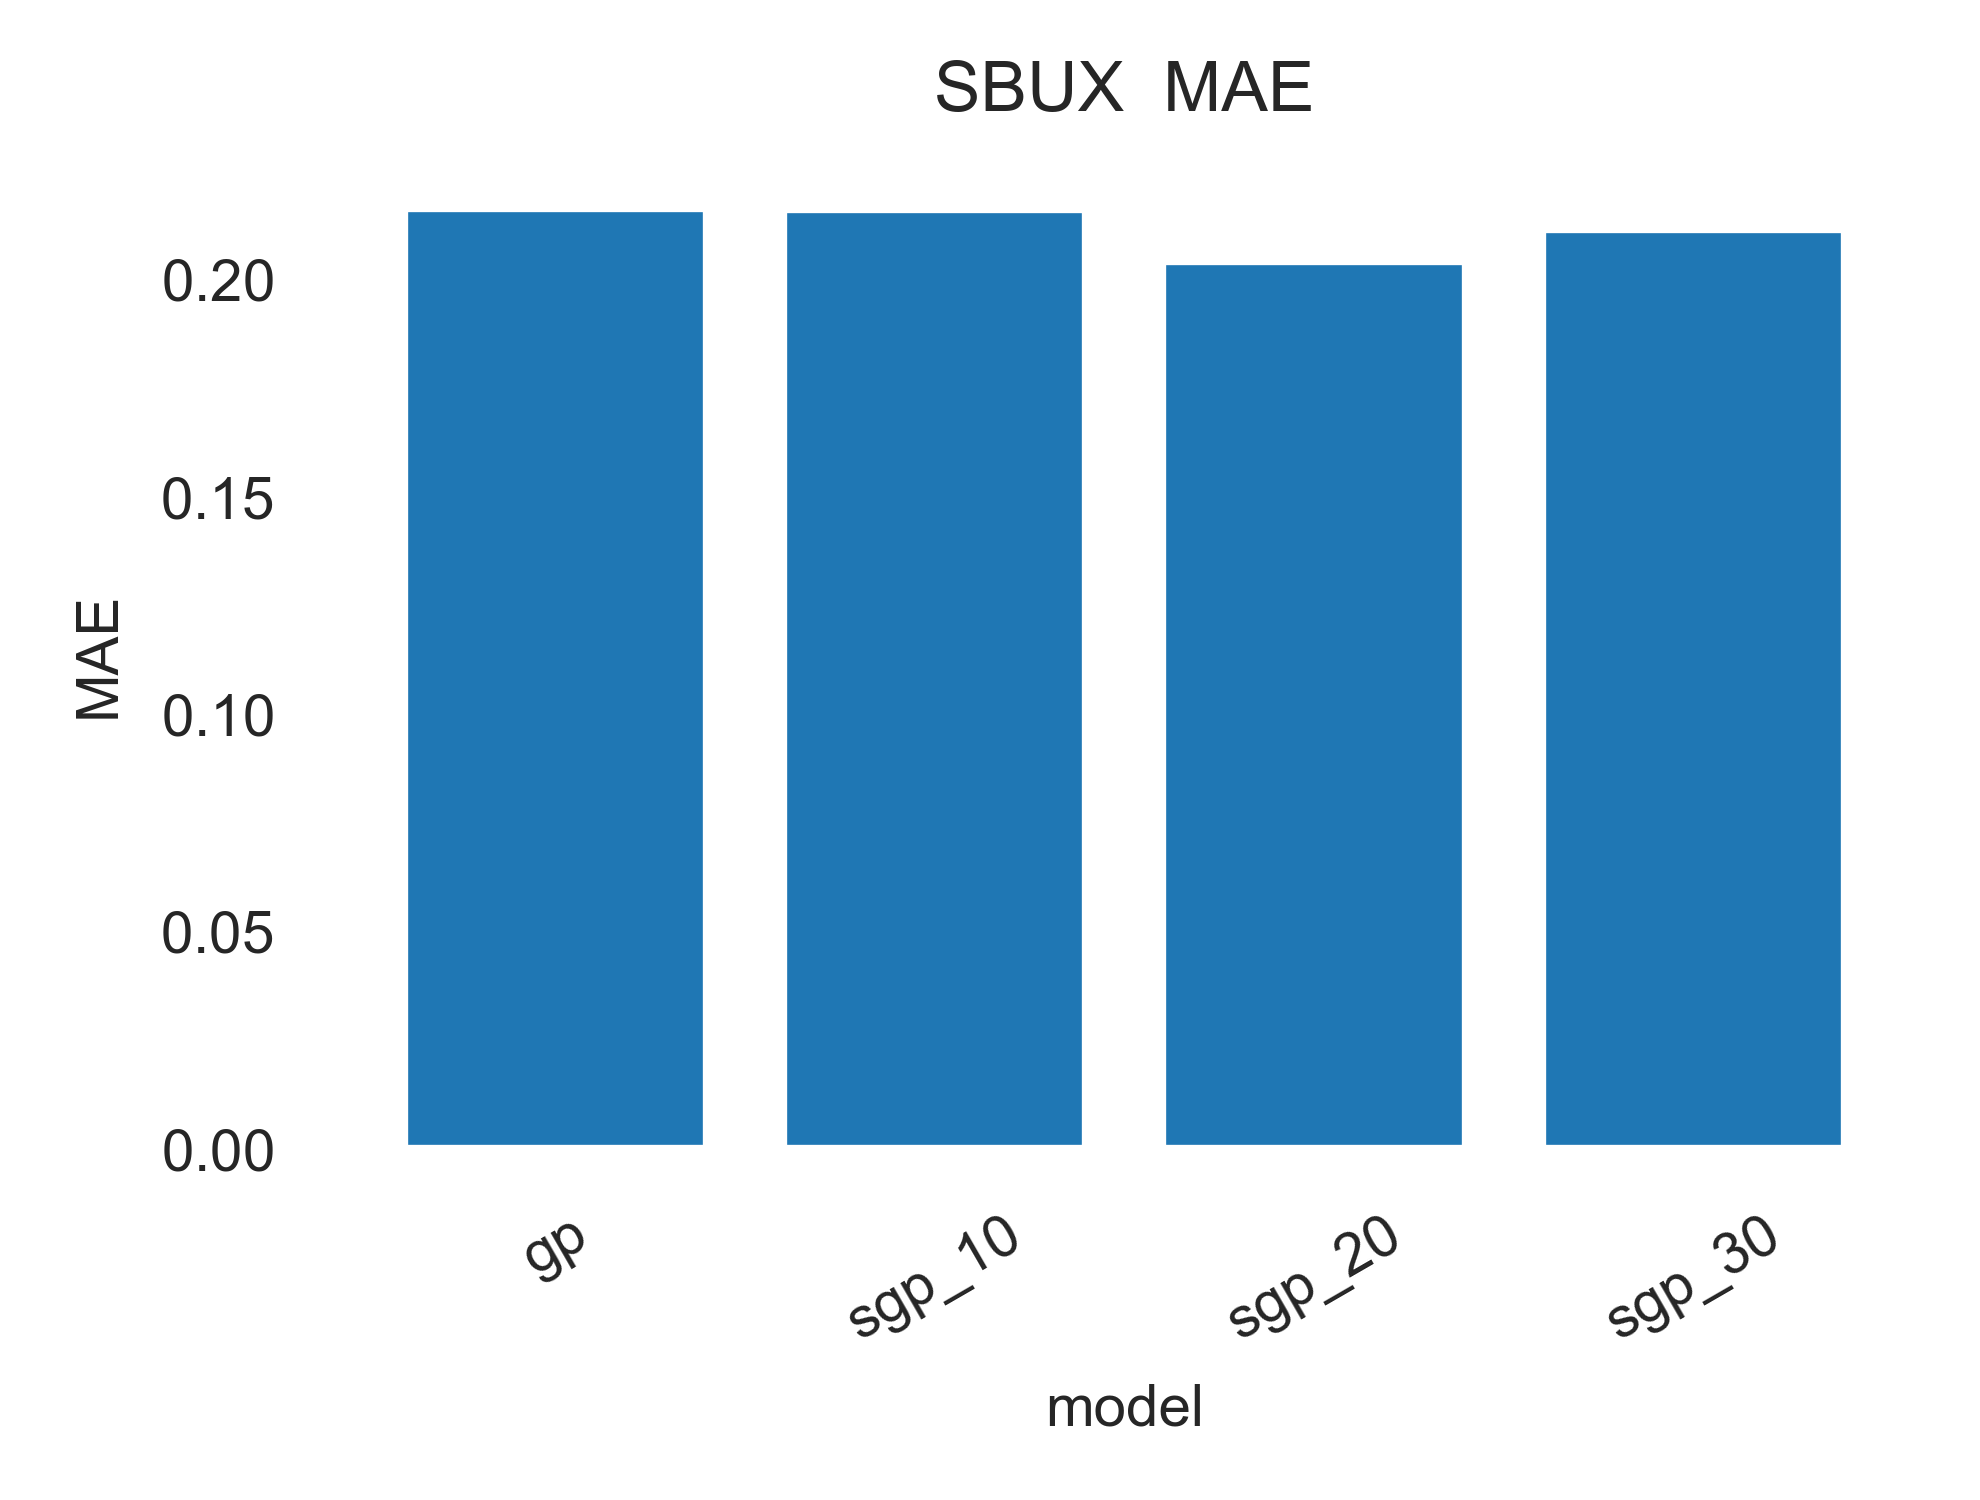
\includegraphics[width=\textwidth]{images/lab3/SBUX_MAE.png}
    \caption{模型滑动预测SBUX时的推理时间}\label{3SBUXMAE}
    \end{minipage}
\end{figure}
